% $Header: /cvsroot/latex-beamer/latex-beamer/solutions/generic-talks/generic-ornate-15min-45min.en.tex,v 1.5 2007/01/28 20:48:23 tantau Exp $

\documentclass[red,compress,xcolor=table]{beamer}

% This file is a solution template for:

% - Giving a talk on some subject.
% - The talk is between 15min and 45min long.
% - Style is ornate.



% Copyright 2004 by Till Tantau <tantau@users.sourceforge.net>.
%
% In principle, this file can be redistributed and/or modified under
% the terms of the GNU Public License, version 2.
%
% However, this file is supposed to be a template to be modified
% for your own needs. For this reason, if you use this file as a
% template and not specifically distribute it as part of a another
% package/program, I grant the extra permission to freely copy and
% modify this file as you see fit and even to delete this copyright
% notice. 


\mode<presentation>
{
  %\usetheme{Warsaw}
  \usetheme{Warsaw}
  %\usecolortheme{lily}
  \usetheme{Frankfurt}

  % or ...
  %\useoutertheme{split}

  \setbeamercovered{transparent}
  %\pagestyle{plain}
  \setbeamerfont*{frametitle}{size=\normalsize,series=\bfseries}
  \setbeamertemplate{navigation symbols}{$\circ$}                      

  % or whatever (possibly just delete it)
}

\usepackage[english]{babel}
% or whatever
\usepackage[dvips]{}

\usepackage[latin1]{inputenc}
% or whatever

\usepackage{tabularx,colortbl}

\usepackage{times}
\usepackage[T1]{fontenc}

\usepackage{wasysym}
\usepackage{url}
\usepackage{grffile}

\usepackage[table]{xcolor}

\newcommand{\bbar}{$\bar{\text{b}}\;$}
\newcommand{\cbar}{$\bar{\text{c}}\;$}
\newcommand{\sbar}{$\bar{\text{s}}\;$}
\newcommand{\tbar}{$\bar{\text{t}}\;$}

\newcommand{\putat}[3]{\begin{picture}(0,0)(0,0)\put(#1,#2){#3}\end{picture}}

\DefineNamedColor{named}{GreenYellow}   {cmyk}{0.15,0,0.69,0}
\DefineNamedColor{named}{Yellow}        {cmyk}{0,0,1,0}
\DefineNamedColor{named}{Goldenrod}     {cmyk}{0,0.10,0.84,0}
\DefineNamedColor{named}{Dandelion}     {cmyk}{0,0.29,0.84,0}
\DefineNamedColor{named}{Apricot}       {cmyk}{0,0.32,0.52,0}
\DefineNamedColor{named}{Peach}         {cmyk}{0,0.50,0.70,0}
\DefineNamedColor{named}{Melon}         {cmyk}{0,0.46,0.50,0}
\DefineNamedColor{named}{YellowOrange}  {cmyk}{0,0.42,1,0}
\DefineNamedColor{named}{Orange}        {cmyk}{0,0.61,0.87,0}
\DefineNamedColor{named}{BurntOrange}   {cmyk}{0,0.51,1,0}
\DefineNamedColor{named}{Bittersweet}   {cmyk}{0,0.75,1,0.24}
\DefineNamedColor{named}{RedOrange}     {cmyk}{0,0.77,0.87,0}
\DefineNamedColor{named}{Mahogany}      {cmyk}{0,0.85,0.87,0.35}
\DefineNamedColor{named}{Maroon}        {cmyk}{0,0.87,0.68,0.32}
\DefineNamedColor{named}{BrickRed}      {cmyk}{0,0.89,0.94,0.28}
\DefineNamedColor{named}{Red}           {cmyk}{0,1,1,0}
\DefineNamedColor{named}{OrangeRed}     {cmyk}{0,1,0.50,0}
\DefineNamedColor{named}{RubineRed}     {cmyk}{0,1,0.13,0}
\DefineNamedColor{named}{WildStrawberry}{cmyk}{0,0.96,0.39,0}
\DefineNamedColor{named}{Salmon}        {cmyk}{0,0.53,0.38,0}
\DefineNamedColor{named}{CarnationPink} {cmyk}{0,0.63,0,0}
\DefineNamedColor{named}{Magenta}       {cmyk}{0,1,0,0}
\DefineNamedColor{named}{VioletRed}     {cmyk}{0,0.81,0,0}
\DefineNamedColor{named}{Rhodamine}     {cmyk}{0,0.82,0,0}
\DefineNamedColor{named}{Mulberry}      {cmyk}{0.34,0.90,0,0.02}
\DefineNamedColor{named}{RedViolet}     {cmyk}{0.07,0.90,0,0.34}
\DefineNamedColor{named}{Fuchsia}       {cmyk}{0.47,0.91,0,0.08}
\DefineNamedColor{named}{Lavender}      {cmyk}{0,0.48,0,0}
\DefineNamedColor{named}{Thistle}       {cmyk}{0.12,0.59,0,0}
\DefineNamedColor{named}{Orchid}        {cmyk}{0.32,0.64,0,0}
\DefineNamedColor{named}{DarkOrchid}    {cmyk}{0.40,0.80,0.20,0}
\DefineNamedColor{named}{Purple}        {cmyk}{0.45,0.86,0,0}
\DefineNamedColor{named}{Plum}          {cmyk}{0.50,1,0,0}
\DefineNamedColor{named}{Violet}        {cmyk}{0.79,0.88,0,0}
\DefineNamedColor{named}{RoyalPurple}   {cmyk}{0.75,0.90,0,0}
\DefineNamedColor{named}{BlueViolet}    {cmyk}{0.86,0.91,0,0.04}
\DefineNamedColor{named}{Periwinkle}    {cmyk}{0.57,0.55,0,0}
\DefineNamedColor{named}{CadetBlue}     {cmyk}{0.62,0.57,0.23,0}
\DefineNamedColor{named}{CornflowerBlue}{cmyk}{0.65,0.13,0,0}
\DefineNamedColor{named}{MidnightBlue}  {cmyk}{0.98,0.13,0,0.43}
\DefineNamedColor{named}{NavyBlue}      {cmyk}{0.94,0.54,0,0}
\DefineNamedColor{named}{RoyalBlue}     {cmyk}{1,0.50,0,0}
\DefineNamedColor{named}{Blue}          {cmyk}{1,1,0,0}
\DefineNamedColor{named}{Cerulean}      {cmyk}{0.94,0.11,0,0}
\DefineNamedColor{named}{Cyan}          {cmyk}{1,0,0,0}
\DefineNamedColor{named}{ProcessBlue}   {cmyk}{0.96,0,0,0}
\DefineNamedColor{named}{SkyBlue}       {cmyk}{0.62,0,0.12,0}
\DefineNamedColor{named}{Turquoise}     {cmyk}{0.85,0,0.20,0}
\DefineNamedColor{named}{TealBlue}      {cmyk}{0.86,0,0.34,0.02}
\DefineNamedColor{named}{Aquamarine}    {cmyk}{0.82,0,0.30,0}
\DefineNamedColor{named}{BlueGreen}     {cmyk}{0.85,0,0.33,0}
\DefineNamedColor{named}{Emerald}       {cmyk}{1,0,0.50,0}
\DefineNamedColor{named}{JungleGreen}   {cmyk}{0.99,0,0.52,0}
\DefineNamedColor{named}{SeaGreen}      {cmyk}{0.69,0,0.50,0}
\DefineNamedColor{named}{Green}         {cmyk}{1,0,1,0}
\DefineNamedColor{named}{ForestGreen}   {cmyk}{0.91,0,0.88,0.12}
\DefineNamedColor{named}{PineGreen}     {cmyk}{0.92,0,0.59,0.25}
\DefineNamedColor{named}{LimeGreen}     {cmyk}{0.50,0,1,0}
\DefineNamedColor{named}{YellowGreen}   {cmyk}{0.44,0,0.74,0}
\DefineNamedColor{named}{SpringGreen}   {cmyk}{0.26,0,0.76,0}
\DefineNamedColor{named}{OliveGreen}    {cmyk}{0.64,0,0.95,0.40}
\DefineNamedColor{named}{RawSienna}     {cmyk}{0,0.72,1,0.45}
\DefineNamedColor{named}{Sepia}         {cmyk}{0,0.83,1,0.70}
\DefineNamedColor{named}{Brown}         {cmyk}{0,0.81,1,0.60}
\DefineNamedColor{named}{Tan}           {cmyk}{0.14,0.42,0.56,0}
\DefineNamedColor{named}{Gray}          {cmyk}{0,0,0,0.50}
\DefineNamedColor{named}{Black}         {cmyk}{0,0,0,1}
\DefineNamedColor{named}{White}         {cmyk}{0,0,0,0}


% Or whatever. Note that the encoding and the font should match. If T1
% does not look nice, try deleting the line with the fontenc.

\begingroup
	\def\facewith#1{$\bigcirc\mskip-13.3mu{}^{..}
	\mskip-11mu\scriptscriptstyle#1\ $}
	\xdef\frowny{\facewith\frown}
	\xdef\smiley{\facewith\smile}
	\xdef\neutry{\facewith-}
\endgroup

\title[VBF Higgs invisible] % (optional, use only with long paper titles)
{Introduction for Long Exercise on Higgs Invisible}

\subtitle
{} % (optional)

\author[A.-M. Magnan] % (optional, use only with lots of authors)
{A.-M. Magnan,
IC London \\
P. Meridiani, Roma }
% - Use the \inst{?} command only if the authors have different
%   affiliation.

\date[CMSDAS@Bari, 20/01/2015] % (optional)
{20/01/2015, CMSDAS@Bari}
%IC $H \rightarrow \tau \tau$ analysis meeting
%SMP-VJ Meeting
%TKCO Meeting

\subject{Talks}
% This is only inserted into the PDF information catalog. Can be left
% out. 



% If you have a file called "university-logo-filename.xxx", where xxx
% is a graphic format that can be processed by latex or pdflatex,
% resp., then you can add a logo as follows:

% \pgfdeclareimage[height=0.5cm]{university-logo}{university-logo-filename}
% \logo{\pgfuseimage{university-logo}}



% Delete this, if you do not want the table of contents to pop up at
% the beginning of each subsection:
%\AtBeginSection[]
%{
%  \begin{frame}<beamer>{Outline}
%    \tableofcontents[currentsection]%,currentsubsection]
%  \end{frame}
%}


% If you wish to uncover everything in a step-wise fashion, uncomment
% the following command: 

%\beamerdefaultoverlayspecification{<+->}


\begin{document}


\begin{frame}
  \titlepage
\end{frame}


\begin{frame}
\frametitle{References to analyses done/ongoing with run I data}

\begin{itemize}
\item \scriptsize Published analysis: \url{http://cms.cern.ch/iCMS/analysisadmin/cadilines?id=1355&ancode=HIG-13-030&line=HIG-13-030}
\item \scriptsize Pre-approved with parked data:\url{http://cms.cern.ch/iCMS/analysisadmin/cadilines?id=1355&ancode=HIG-14-038&line=HIG-14-038} 
\item \scriptsize and analysis notes connected to these CADI entries.
\item \scriptsize In this exercise: will concentrate on the VBF production only.
\end{itemize}

\begin{block}{\centering Many thanks to ...}
\begin{itemize}
\item \scriptsize \textcolor{Salmon}{Chayanit Asawatangtrakuldee}: the main analyser for \textcolor{Salmon}{published analysis}.
\item \scriptsize \textcolor{Blue}{Patrick Dunne}: the main analyser for \textcolor{Blue}{parked data analysis}.
\item \scriptsize \textcolor{ForestGreen}{Renjie Wang} for sharing his code to convert the limit to \textcolor{ForestGreen}{Dark Matter models}.
\item \scriptsize ... and the rest of the Higgs invisible team.
\end{itemize}
\end{block}


\end{frame}

\begin{frame}
\frametitle{Higgs to invisible production in Vector Boson Fusion mode}

\begin{columns}
  \column{0.6\textwidth}
\begin{itemize}
\item \scriptsize Higher cross-section than VH associated production mechanisms.
\item \scriptsize Final state: 2 jets + missing energy (MET).
\item \scriptsize Main background: QCD !! But, fortunately:
\item \scriptsize no lepton,
\item \scriptsize very characteristic kinematics for the dijet pair: forward-backward with high dijet mass,
\item \scriptsize no hard hadronic activity expected in the rapidity gap between the two jets,
\item \scriptsize large and significant MET.
\item \scriptsize From measured yields: extract 95\% CL limits on the branching ratio to invisible.
\end{itemize}
  \column{0.4\textwidth}
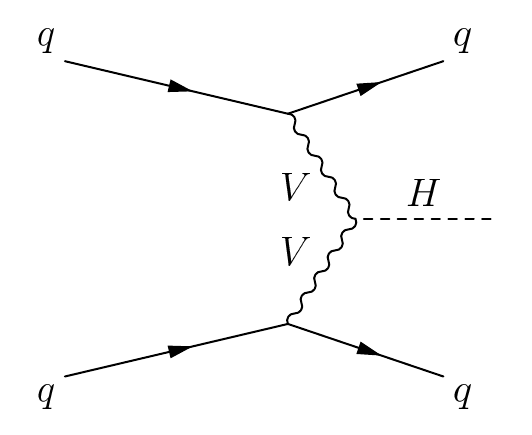
\includegraphics[width=1.0\textwidth]{./qqHqq.png}\\
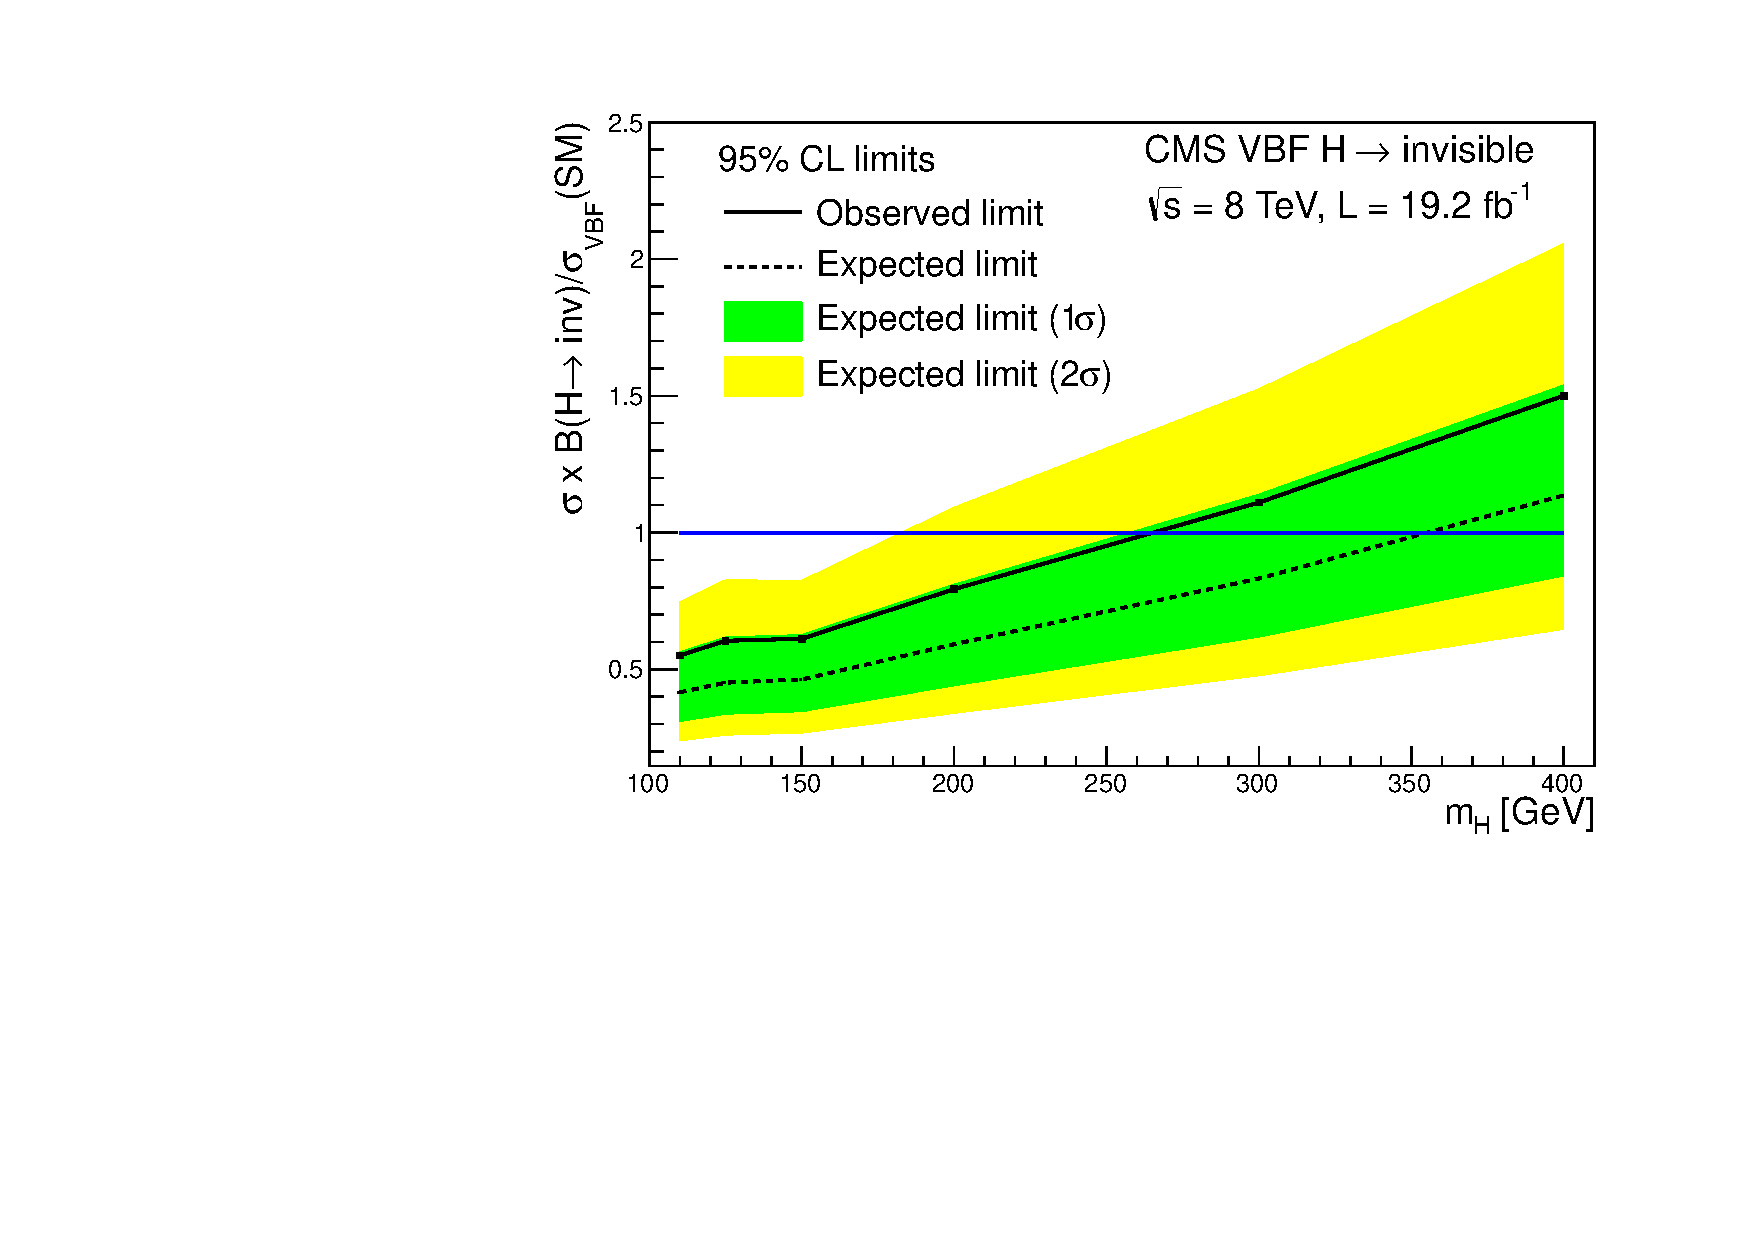
\includegraphics[width=1.0\textwidth]{./vbflimit.pdf}
\end{columns}

\end{frame}

\begin{frame}
\frametitle{Triggers}

\begin{columns}
  \column{0.7\textwidth}
\begin{block}{\scriptsize Run I}
\begin{itemize}
\item \scriptsize L1 seed: ETM40.
\end{itemize}
{\tiny
\begin{tabular}{|l|c|c|c|}
\hline
Run period & MET cut & dijet pT cut & dijet mass cut \\
\hline
A & METnoMuons$>65$ GeV & DiPFJet40 & MJJ800 \\
B\&C &  & DiJet35 & MJJ700 \\
D &  & DiJet30 & MJJ700 \\
\hline
\end{tabular}
}
\end{block}
 \column{0.4\textwidth}
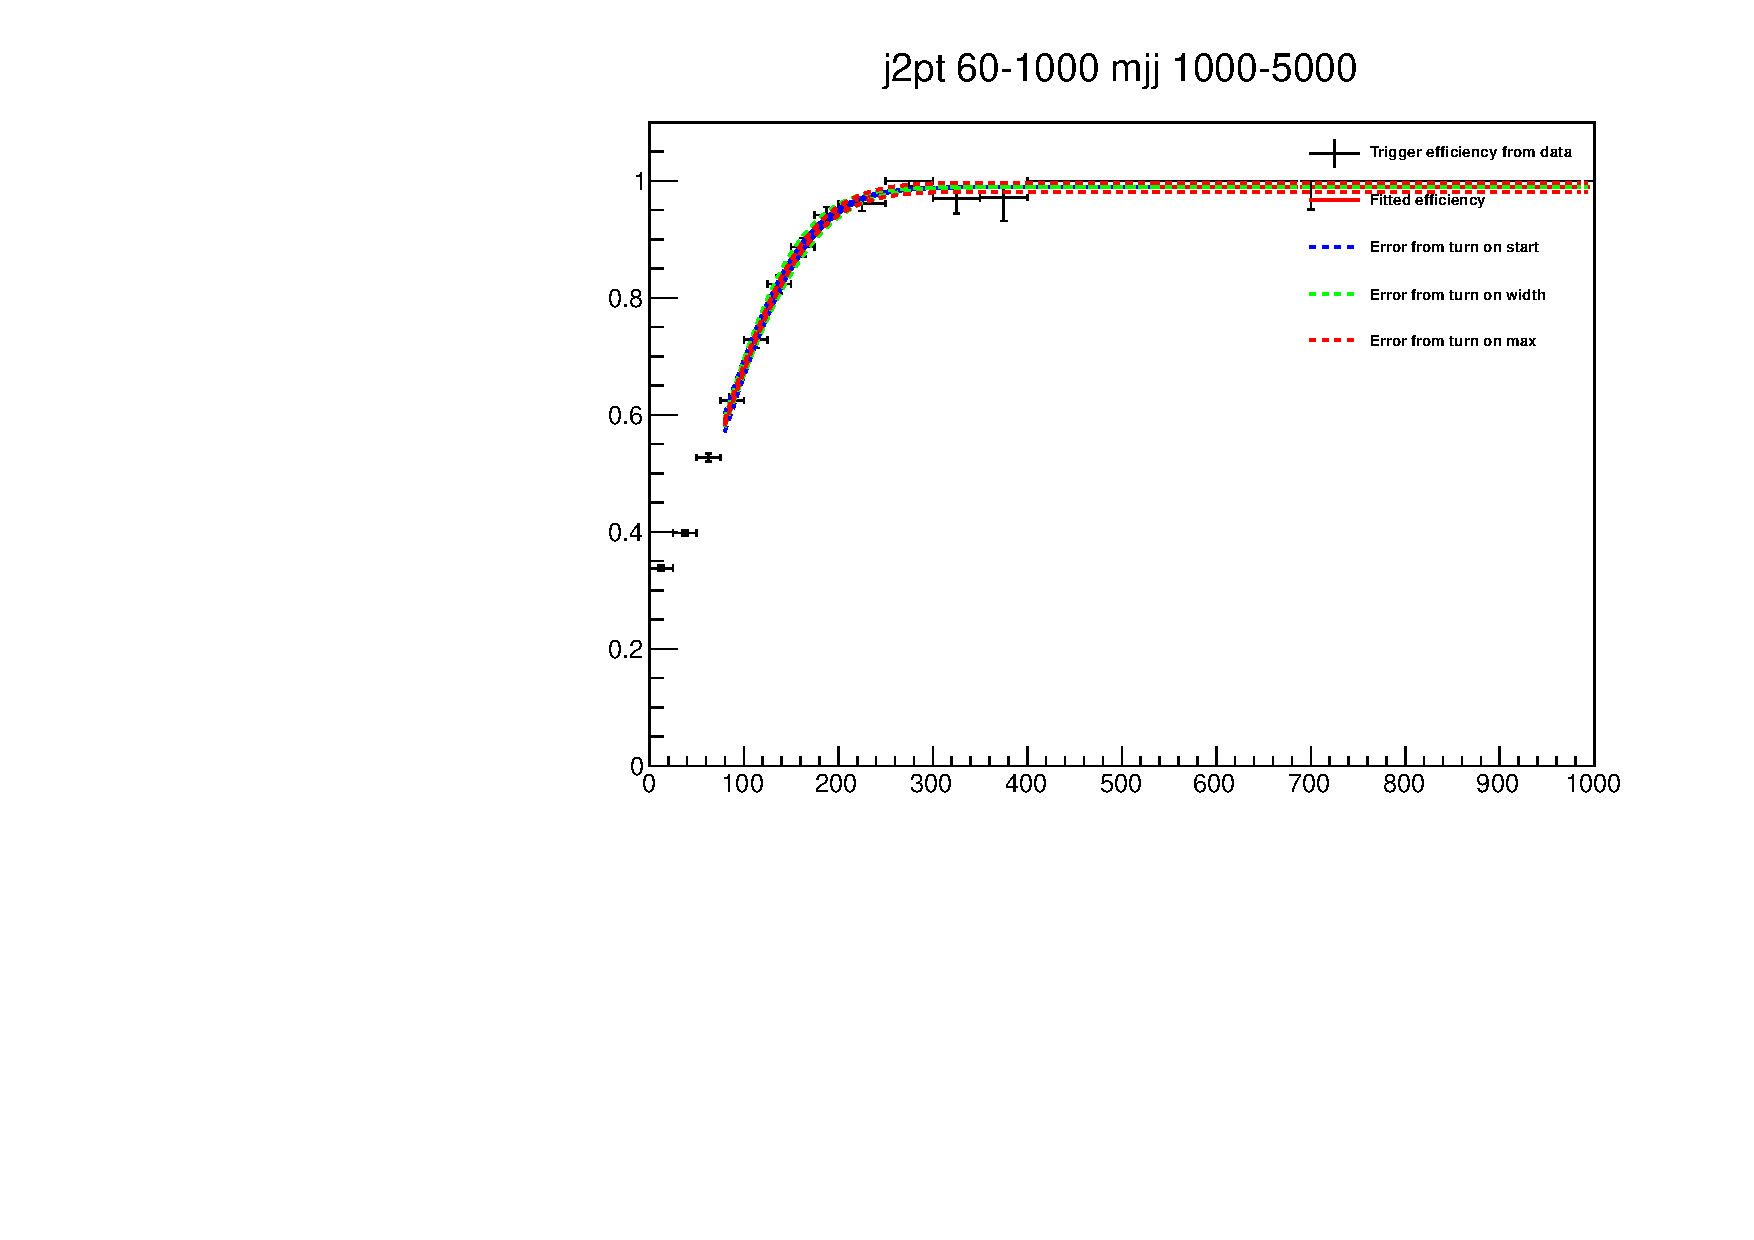
\includegraphics[width=1.0\textwidth]{./hData_MET_1D_45D.pdf}
\end{columns}

\begin{center}
\begin{block}{\scriptsize Proposed for Run II}
\begin{itemize}
\item \scriptsize L1 seed: ETM70.
\item \scriptsize L1 seed for control trigger: ETM50.
\end{itemize}
{\tiny
\begin{tabular}{|l|c|c|c|c|c|}
\hline
Trigger & MET cut & dijet pT cut & dijet mass cut & eff & rate \\
\hline
Baseline & PFMET170 & - & - & 9\% & - \\
VBF & PFMETNoMu140 &  DiPFJetVBF40 & MJJ600 & 10.5\% & 4.7 Hz \\
Control & PFMETNoMu80 &  DiPFJetVBF40 & MJJ600 & 10.5\% & 0.5 Hz \\
\hline
\end{tabular}
}
\end{block}
\end{center}

\putat{280}{115}{\tiny MET (GeV)}

\end{frame}

\begin{frame}
\frametitle{Strategy (1/3)}
\begin{block}{\scriptsize \centering Fiducial and trigger-driven selections for Run I triggers}
\begin{itemize}
\item \scriptsize $|\eta^{j1,j2}|<4.7$, $\eta^{j1}\times \eta^{j2} < 0$, $\Delta\eta_{jj} > 3.6$
\item \scriptsize p$_T^{j1}>50$\,GeV, p$_T^{j2}>40$\,GeV, M$_{jj}>1000$ GeV.
\item \scriptsize PFMETNoMu$>90$\,GeV.
\end{itemize}
\end{block}
\begin{block}{\scriptsize \centering Fiducial and trigger-driven selections for Run II triggers}
\begin{itemize}
\item \scriptsize $|\eta^{j1,j2}|<4.7$, $\eta^{j1}\times \eta^{j2} < 0$, $\Delta\eta_{jj} > 3.6$
\end{itemize}
\begin{columns}
  \column{0.4\textwidth}
\begin{block}{\scriptsize Guesses for Baseline}
\begin{itemize}
\item \scriptsize p$_T^{j1}>30$\,GeV, p$_T^{j2}>30$\,GeV, M$_{jj}>400$ GeV.
\item \scriptsize PFMETNoMu$>250$\,GeV.
\end{itemize}
\end{block}
  \column{0.4\textwidth}
\begin{block}{\scriptsize Guesses for VBF+Control}
\begin{itemize}
\item \scriptsize p$_T^{j1}>50$\,GeV, p$_T^{j2}>50$\,GeV, M$_{jj}>900$ GeV.
\item \scriptsize PFMETNoMu$>200$\,GeV.
\end{itemize}
\end{block}
\end{columns}
\end{block}

\end{frame}

\begin{frame}
\frametitle{After trigger sel: what is our sample composition ?}

\begin{itemize}
\item \scriptsize 99.999\% QCD multijets: mainly fake MET.
\item \scriptsize W+jets, top, VV: real MET from leptonic decays of Ws, lepton(s) not reconstructed (e.g. too soft, outside e/$\mu$ fiducial regions).
\item \scriptsize W+jets, W$\rightarrow\tau_{had}+\nu$: hadronic tau jet either one of the tagging jet or extra jet.
\item \scriptsize Z+jets, Z$\rightarrow \nu\nu$: for this, Z$\rightarrow \mu\mu$ is a great handle. Muons: little calorimetric energy, p$_T$ can be added vectorially to MET to mimic invisible decay.
\item \scriptsize EWK W/Z+2j production: same VBF jet topology.
\end{itemize}

\begin{block}{\scriptsize The METnoMuons subtlety}
\begin{itemize}
\item \scriptsize Will use Z$\rightarrow \mu\mu$ data to estimate Z$\rightarrow \nu\nu$.
\item \scriptsize Need to have stat after trigger: ignore muons when calculating MET.
\item \scriptsize Note: L1MET is also only made with calorimeter towers.
\item \scriptsize Baseline trigger for RunII is not so good for us: will cut a lot of Z$\rightarrow \mu\mu$ statistics.
\end{itemize}
\end{block}


\end{frame}

\begin{frame}
\frametitle{Strategy (2/3)}

\begin{block}{\centering GET RID OF QCD MULTIJET BACKGROUND}
\begin{itemize}
\item \scriptsize MET significance $>4$ (calculated without tight muons).
\item \scriptsize MET isolated from hard jets in $\phi$: min$\Delta\phi$(all jets p$_T>30$ GeV, MET)$>2.0$ (again ignoring tight muons in the MET).
\end{itemize}
\end{block}
\begin{columns}
  \column{0.5\textwidth}
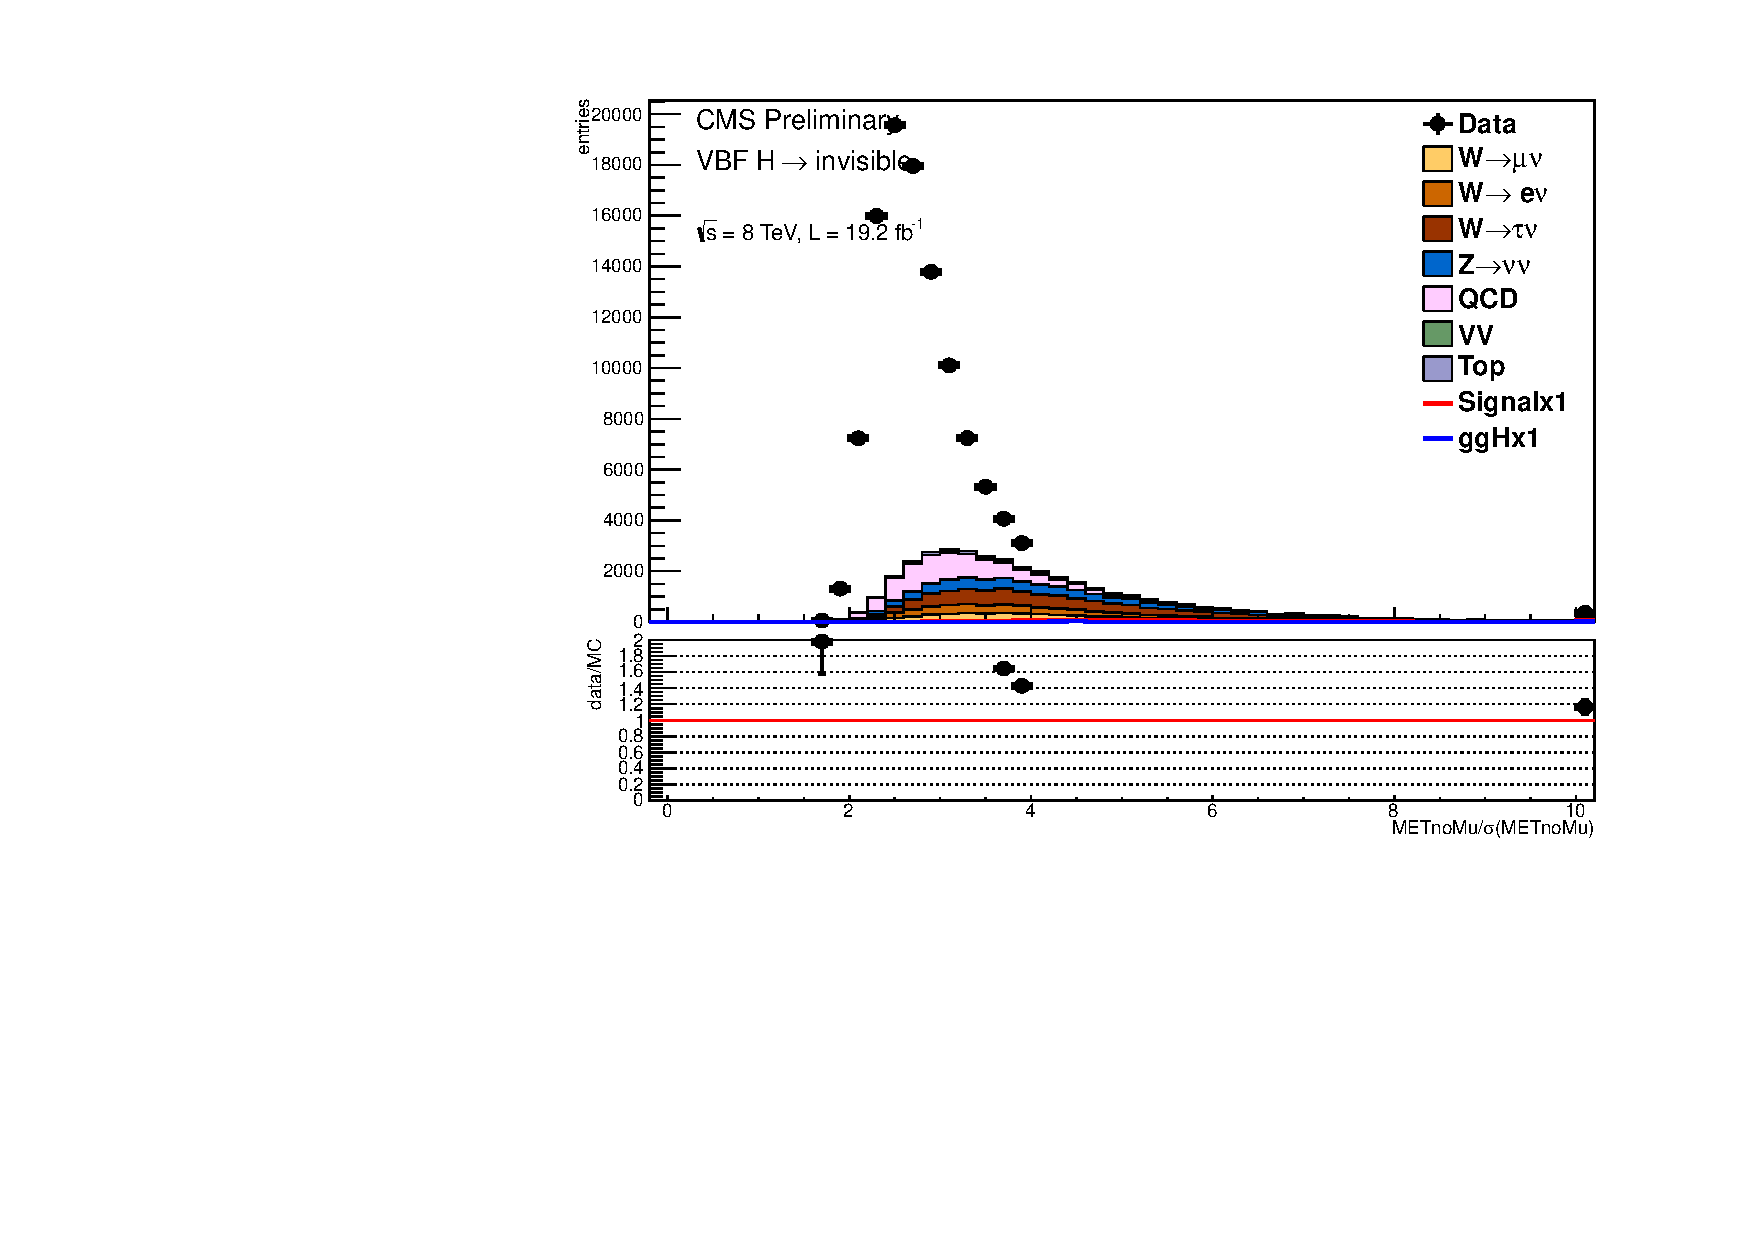
\includegraphics[width=1.0\textwidth]{./nopreselnunu_metnomu_significance.pdf}
  \column{0.5\textwidth}
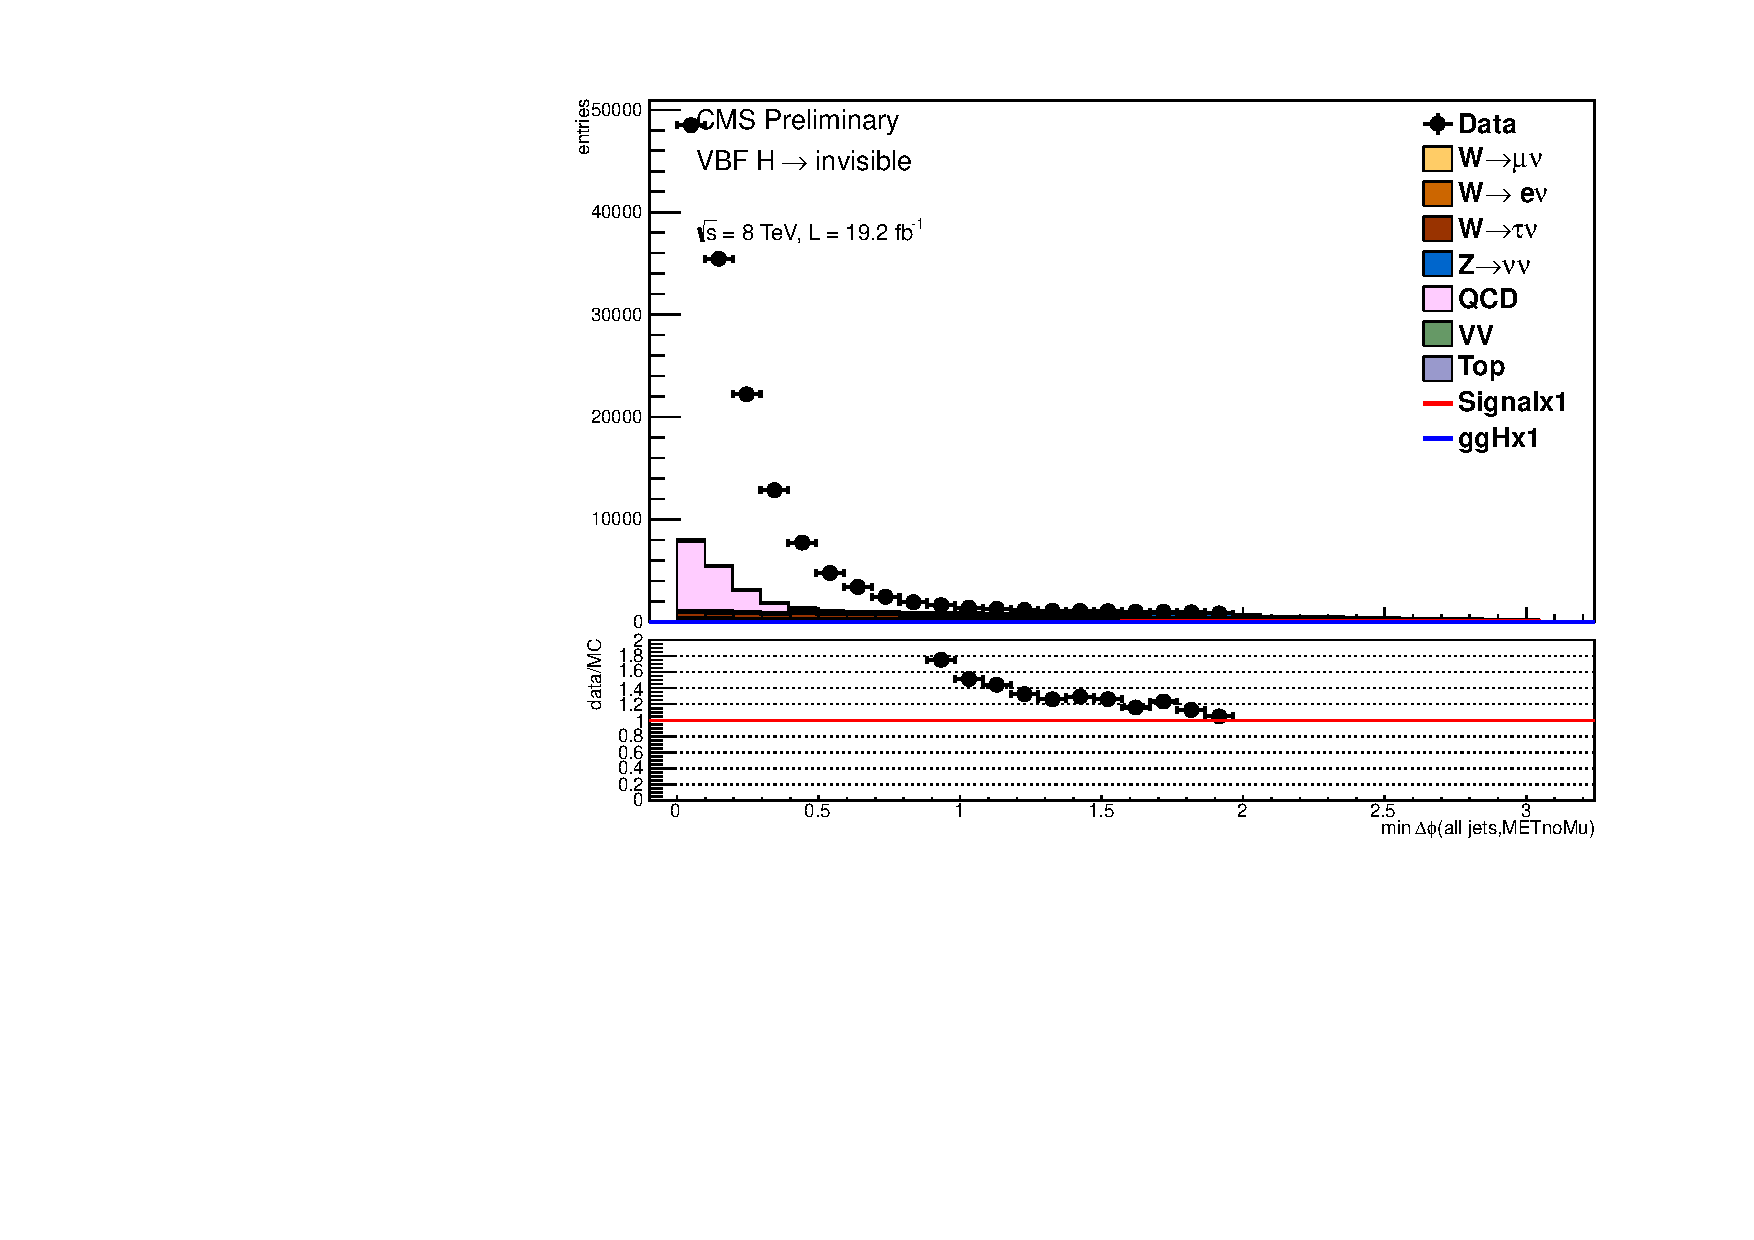
\includegraphics[width=1.0\textwidth]{./metsigpreselnunu_alljetsmetnomu_mindphi.pdf}
\end{columns}

\end{frame}

\begin{frame}
\frametitle{Strategy (3/3)}
\begin{block}{\centering Optimise selection on 95\% CL limit}
\begin{itemize}
\item \scriptsize Blind the analysis.
\item \scriptsize Signal region: apply electron and muon vetos (loose ID, medium isolation).
\item \scriptsize Control regions (see next slides): extract SF to apply on MC with same selection as signal except lepton requirements.
\item \scriptsize Optimise cut-based selection in signal region using rescaled MC: find best cut values for MET significance, min$\Delta\phi$(all jets p$_T>30$ GeV, MET), p$_T^{jets}$, M$_{jj}$.
\item \scriptsize Final figure of merit is the 95\% CL limit.
\item \scriptsize Neglect QCD for the optimisation.
\end{itemize}
\end{block}
\centering 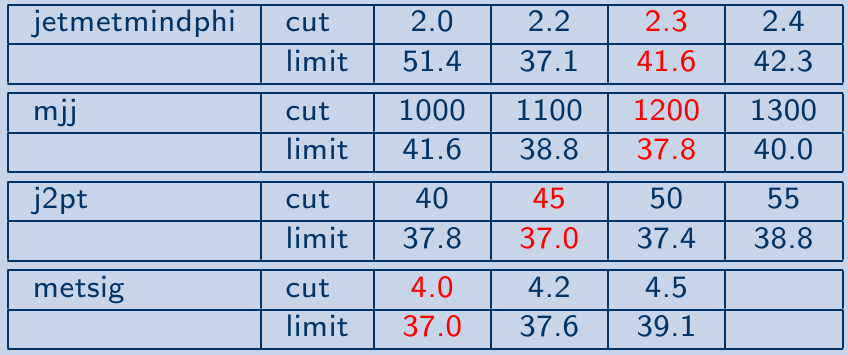
\includegraphics[width=0.6\textwidth]{./tableOptim.png}

\end{frame}

\begin{frame}
\frametitle{Extraction of limits}

\begin{itemize}
\item \scriptsize Simple cut\& count approach: after killing QCD, other backgrounds are too signal like $\Rightarrow$ no improvement from using multivariate techniques.
\item \scriptsize Background estimates: as much as possible rely on data.
\item \scriptsize Use a control region per background:
  \begin{itemize}
  \item \scriptsize W+jets: exactly one lepton (e,$\mu$,$\tau$).
  \item \scriptsize Z+jets: exactly two muons.
  \item \scriptsize top: one electron + one muon.
  \end{itemize}
\item \scriptsize Normalise MC to data in control regions.
\item \scriptsize Check data-MC agreement in shapes in control regions.
\item \scriptsize Extract yields in signal region from normalised MC.
\item \scriptsize Based on agreement in control regions: unblind.
\end{itemize}

\end{frame}

\begin{frame}
\frametitle{Normalisation to control regions}


\begin{block}{\scriptsize Generic equation}
\begin{equation}
  N_{S}^{A}=N_{S}^{A\,MC}\frac{N_{C}^{Data}-N_{C}^{bkg}}{N_{C}^{A\,MC}},
\end{equation}
where
\begin{itemize}
\item \scriptsize $N_{S}^{A}$: number of events from process A in the signal region.
\item \scriptsize $N_{S/C}^{A\,MC}$: number of events predicted by process A Monte Carlo in the signal/control region.
\item \scriptsize $N_{C}^{Data}$: number of data events in the control region.
\item \scriptsize $N_{C}^{Bkg}$: number of events from other background processes in the control region.
\item \scriptsize A = top, W$\rightarrow$e, W$\rightarrow\mu$,W$\rightarrow\tau_{had}$ 
\end{itemize}
\end{block}

\begin{block}{\scriptsize Complication for $\mu\mu$ region}
\begin{equation}
  N_{S}^{Z\rightarrow\nu\nu}=\left(N_{C}^{Data}-N_{C}^{bkg}\right) \cdot\frac{\sigma\left(Z\rightarrow\nu\nu\right)}{\sigma\left(Z\rightarrow\mu\mu\right)}\cdot \frac{\epsilon_{S}^{ZMC}}{\epsilon_{C}^{ZMC}},
\end{equation}
\end{block}

\end{frame}

\begin{frame}
\frametitle{A word on QCD multijet}


\begin{columns}
  \column{0.55\textwidth}
\begin{block}{\scriptsize MC - not enough stat}
\begin{itemize}
\item \scriptsize VBF-enriched: genMET>40 GeV $\Rightarrow$ missing fake MET contribution.
\item \scriptsize Always 3rd jet p$_T>30$ GeV aligned with MET: jet with high neutrino component.
\item \scriptsize Good agreement with data in shape for this population.
\end{itemize}
\begin{columns}
  \column{0.4\textwidth}
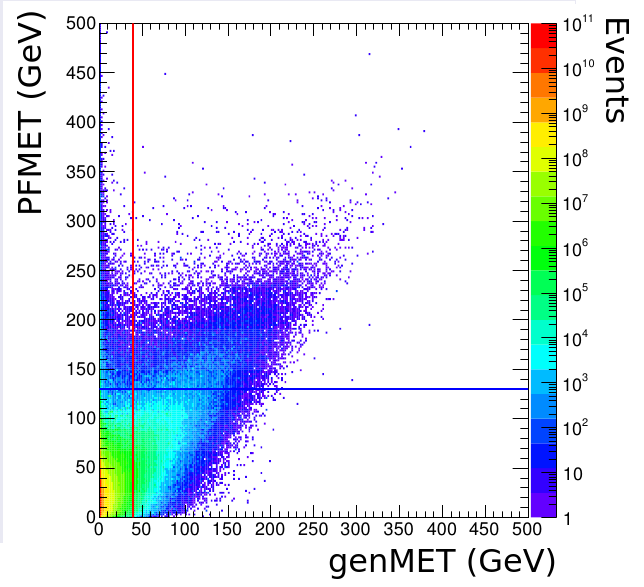
\includegraphics[width=1.2\textwidth]{./Joao_140209_p11.png}
  \column{0.4\textwidth}
\hspace*{-0.5cm}
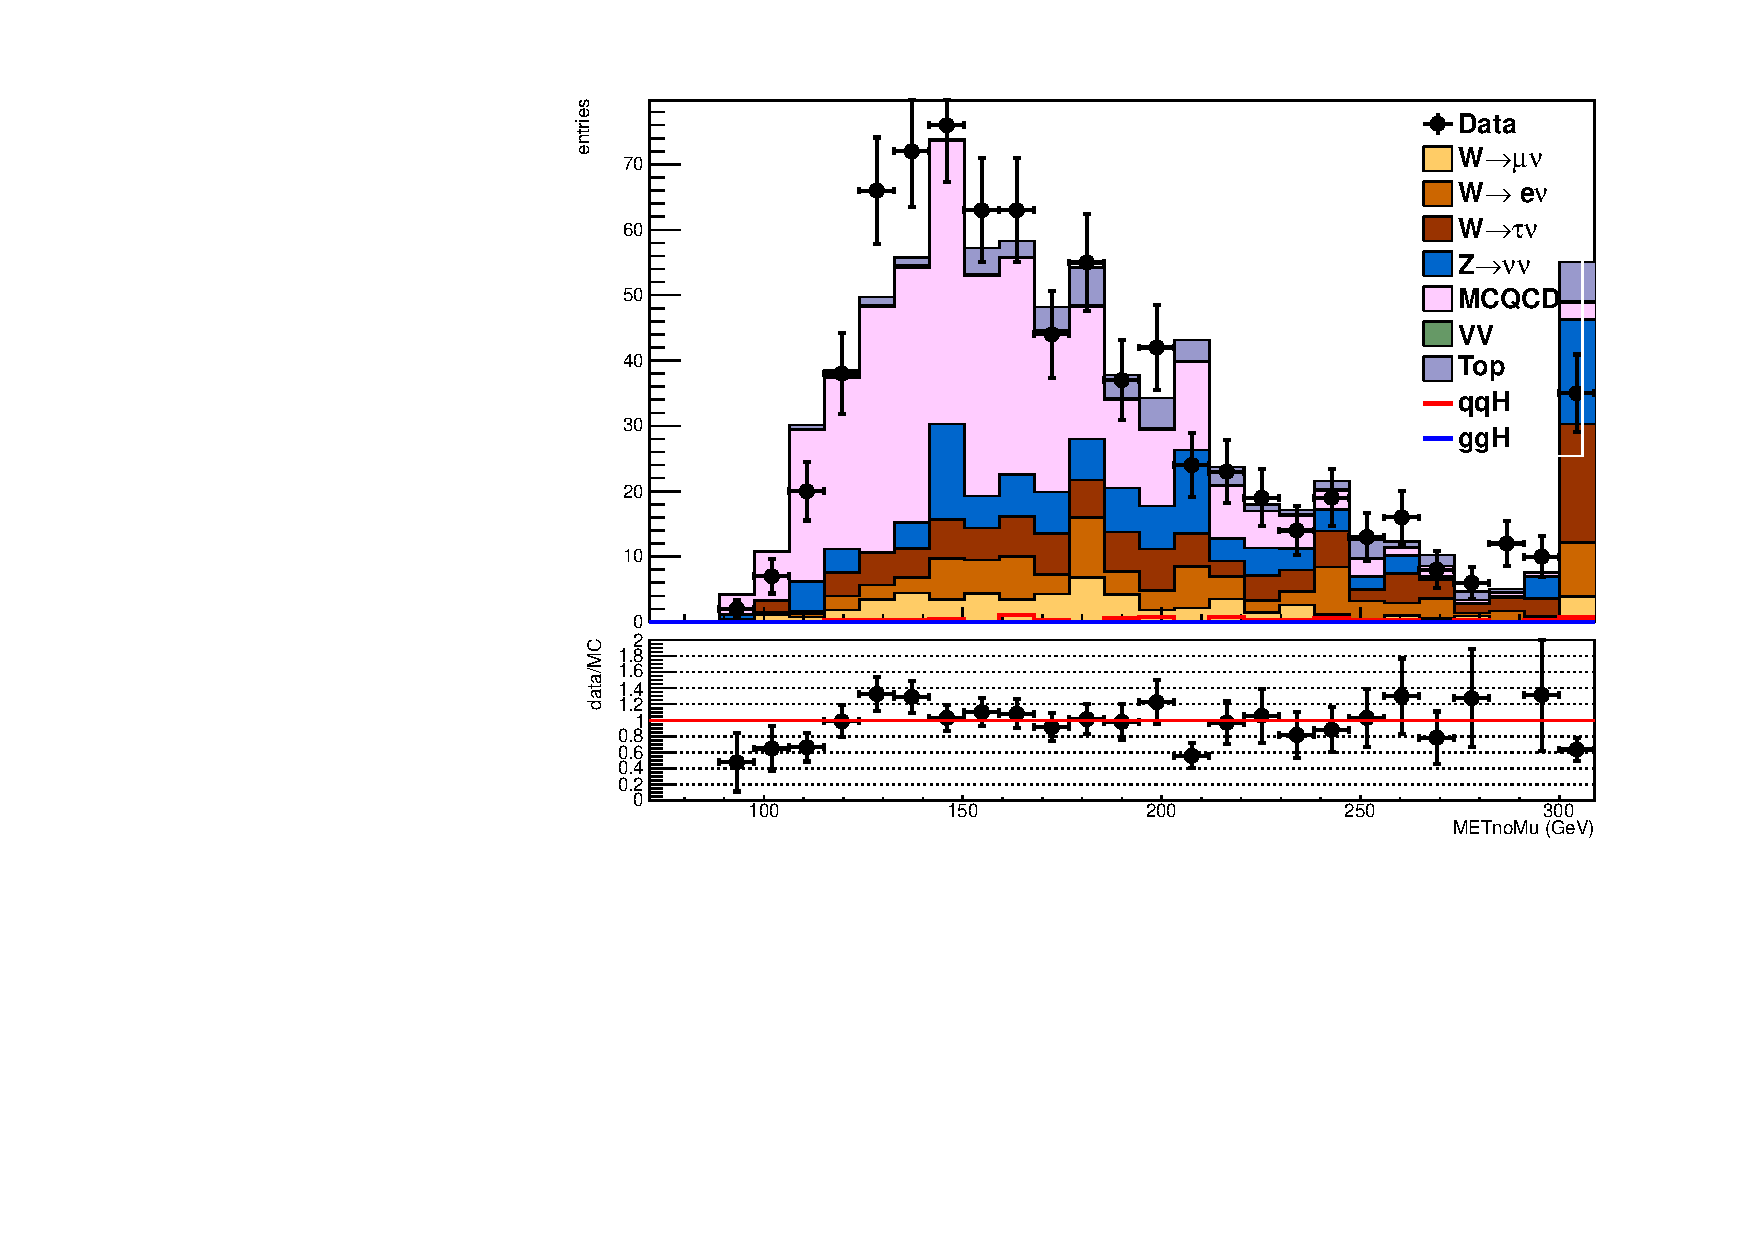
\includegraphics[width=1.2\textwidth]{./qcdinv_qcd_metnomuons.pdf}\\
\hspace*{-0.5cm}
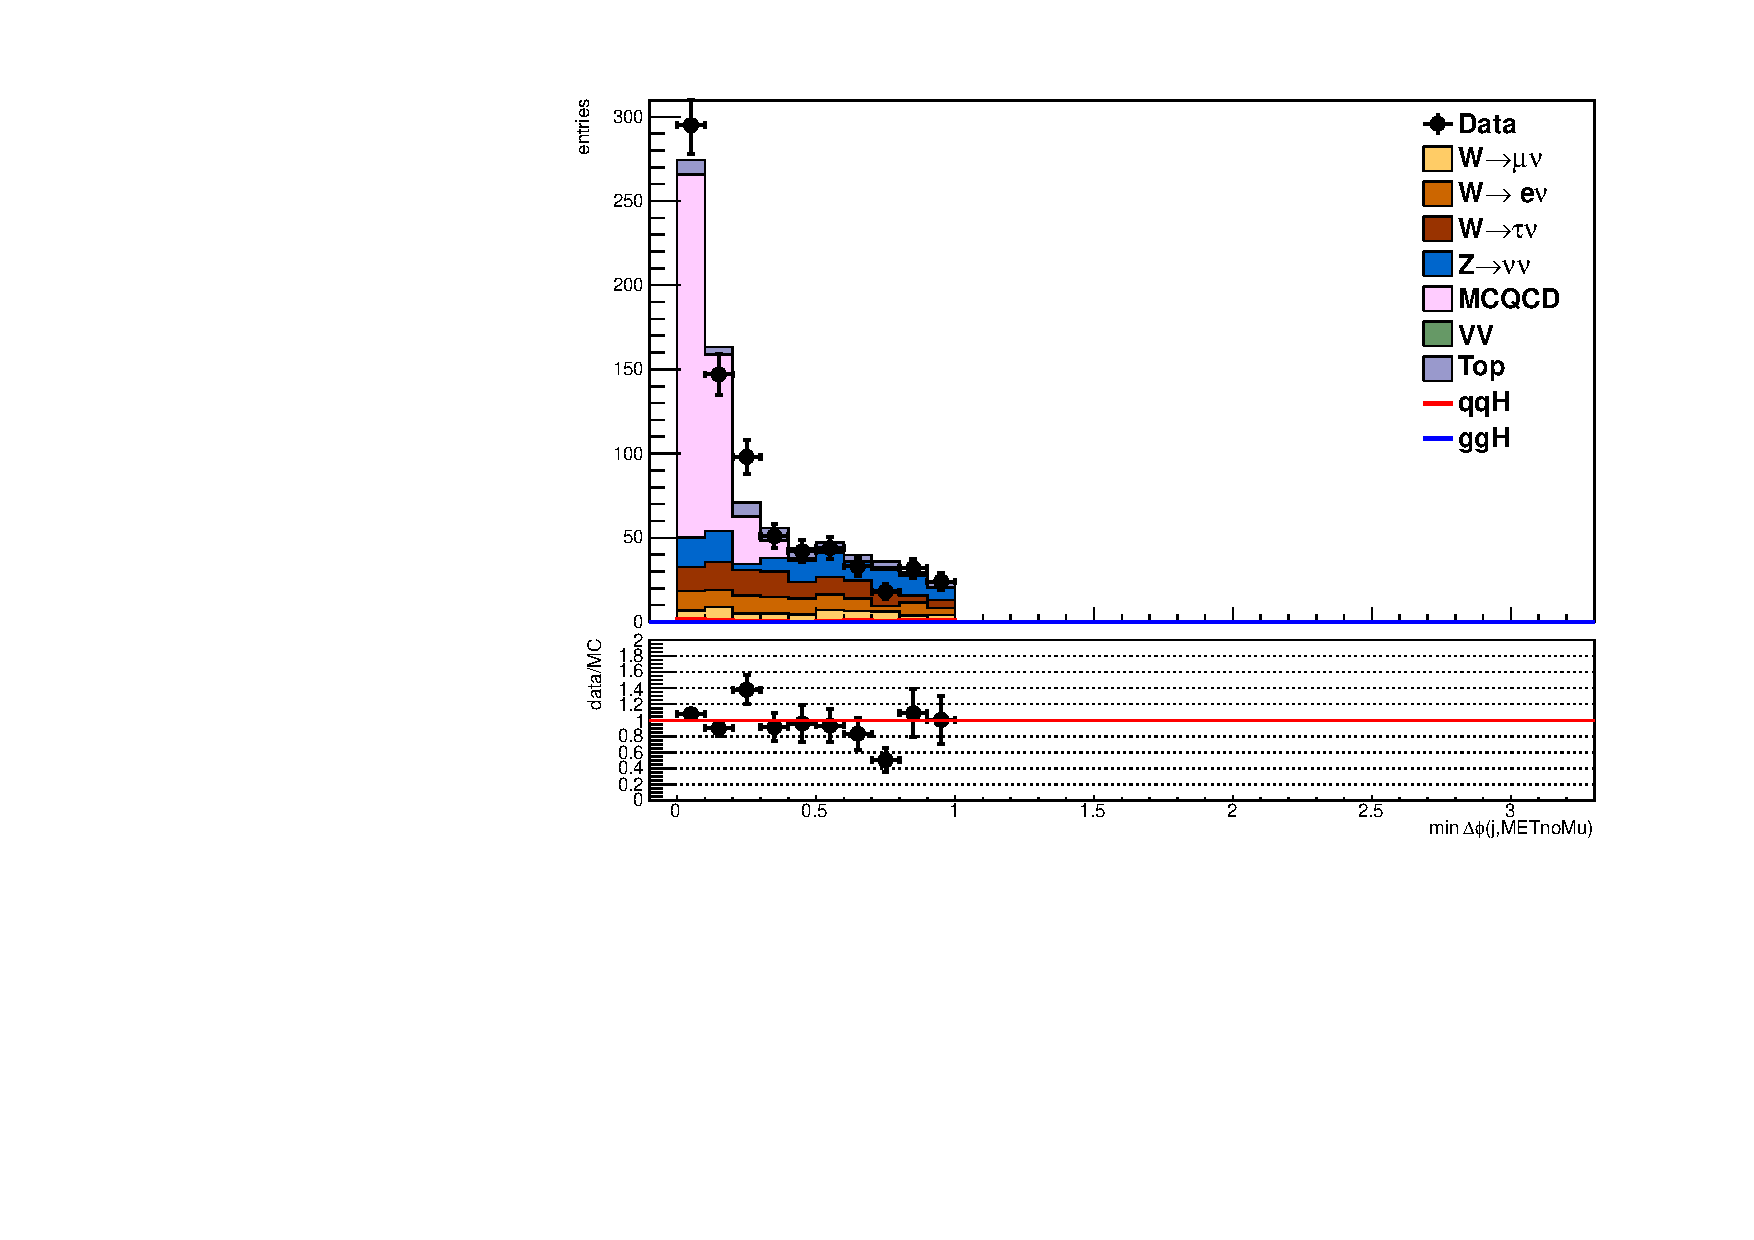
\includegraphics[width=1.2\textwidth]{./qcdinv_qcd_alljetsmetnomu_mindphi.pdf}
\end{columns}
%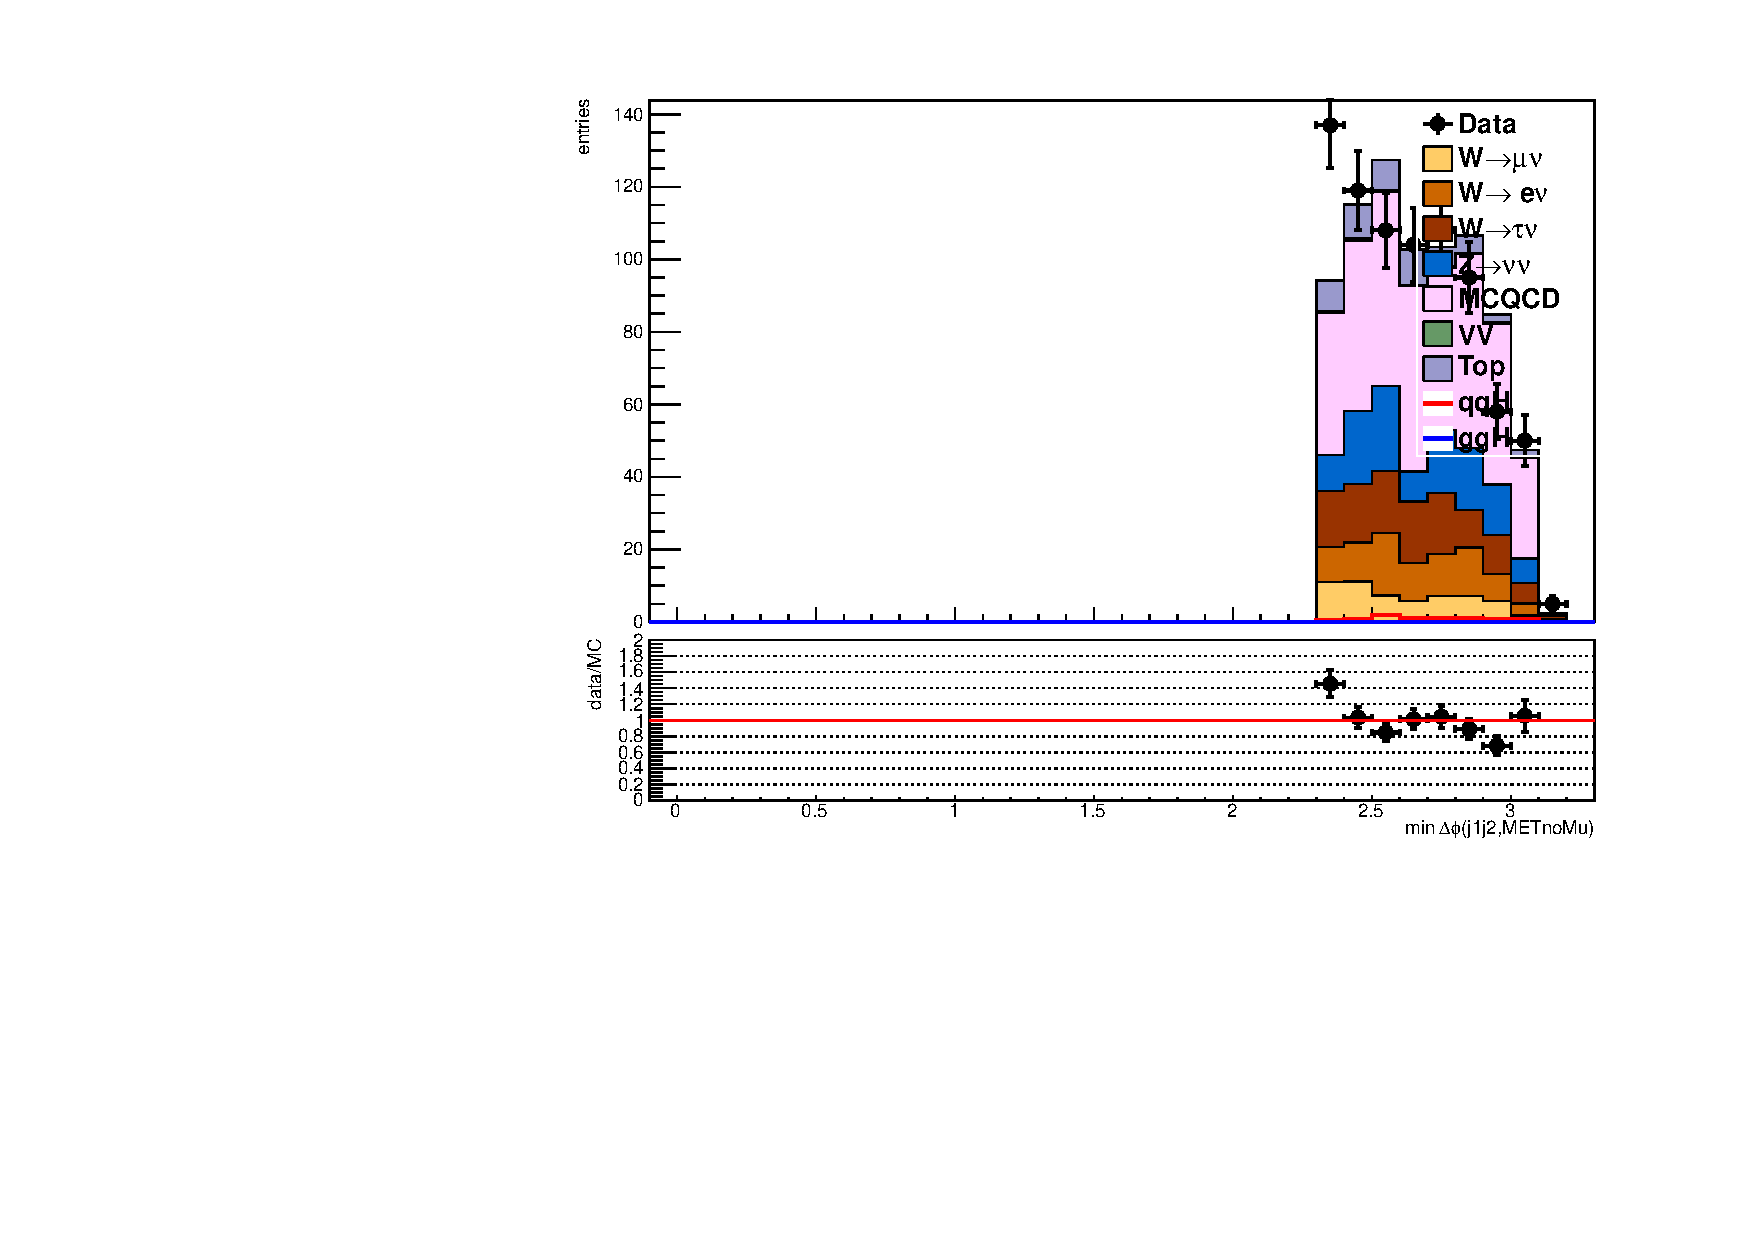
\includegraphics[width=0.5\textwidth]{./qcdinv_qcd_jetmetnomu_mindphi.pdf}

\end{block}
  \column{0.5\textwidth}
\begin{block}{\scriptsize Data-driven - tricky}
\begin{itemize}
\item \scriptsize Use events with non-isolated MET to predict isolated component.
\item \scriptsize ABCD doesn't work: signal contamination too large in 3/4 regions ! Use extrapolations.
\item \scriptsize In the end: small number with large uncertainty $\Rightarrow$ small impact on limit.
\end{itemize}
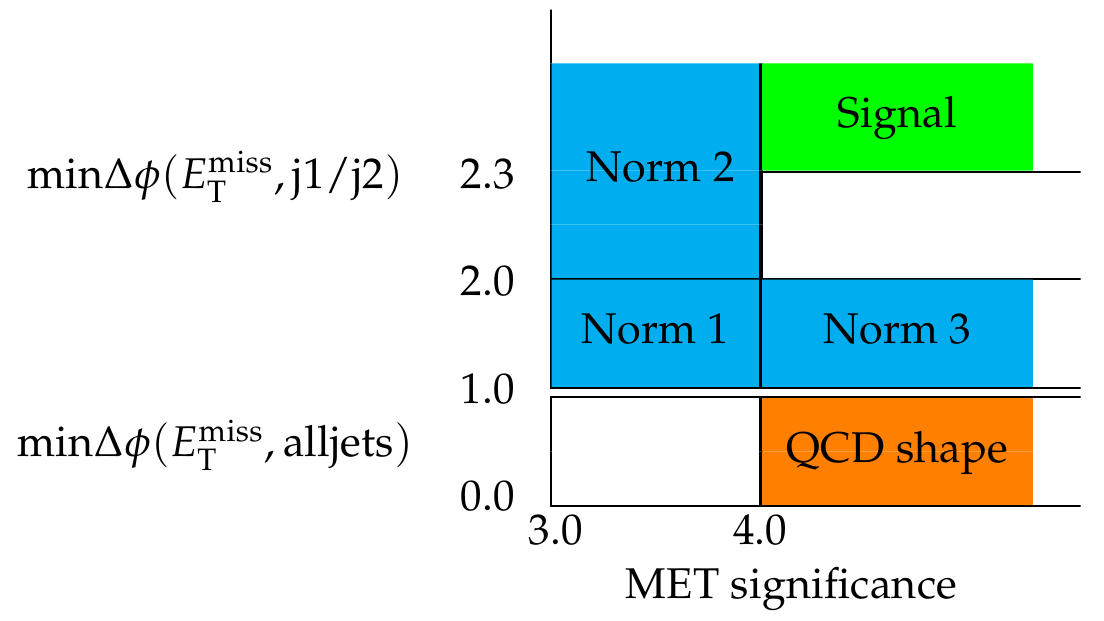
\includegraphics[width=0.5\textwidth]{./schema.png}
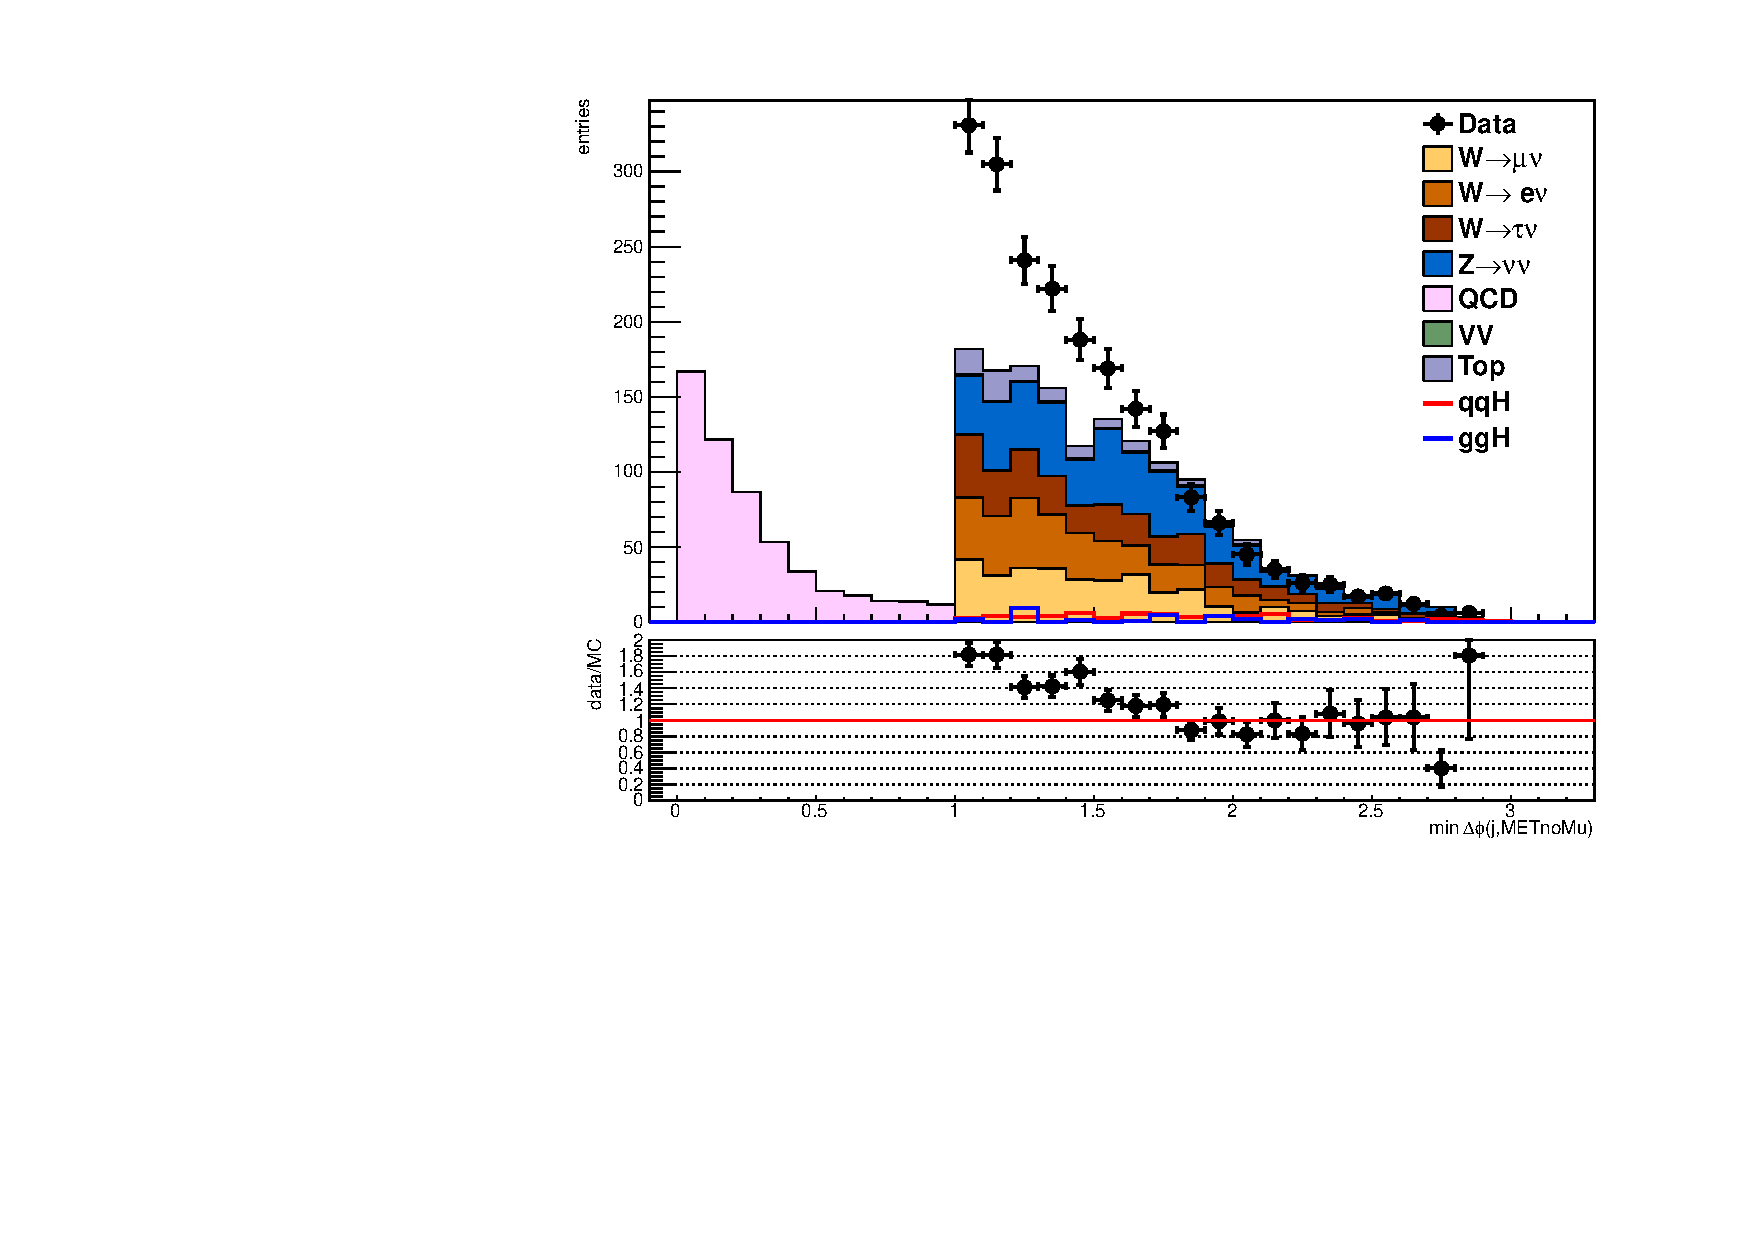
\includegraphics[width=0.5\textwidth]{./qcdinv_3j_nunu_alljetsmetnomu_mindphi.pdf}\\
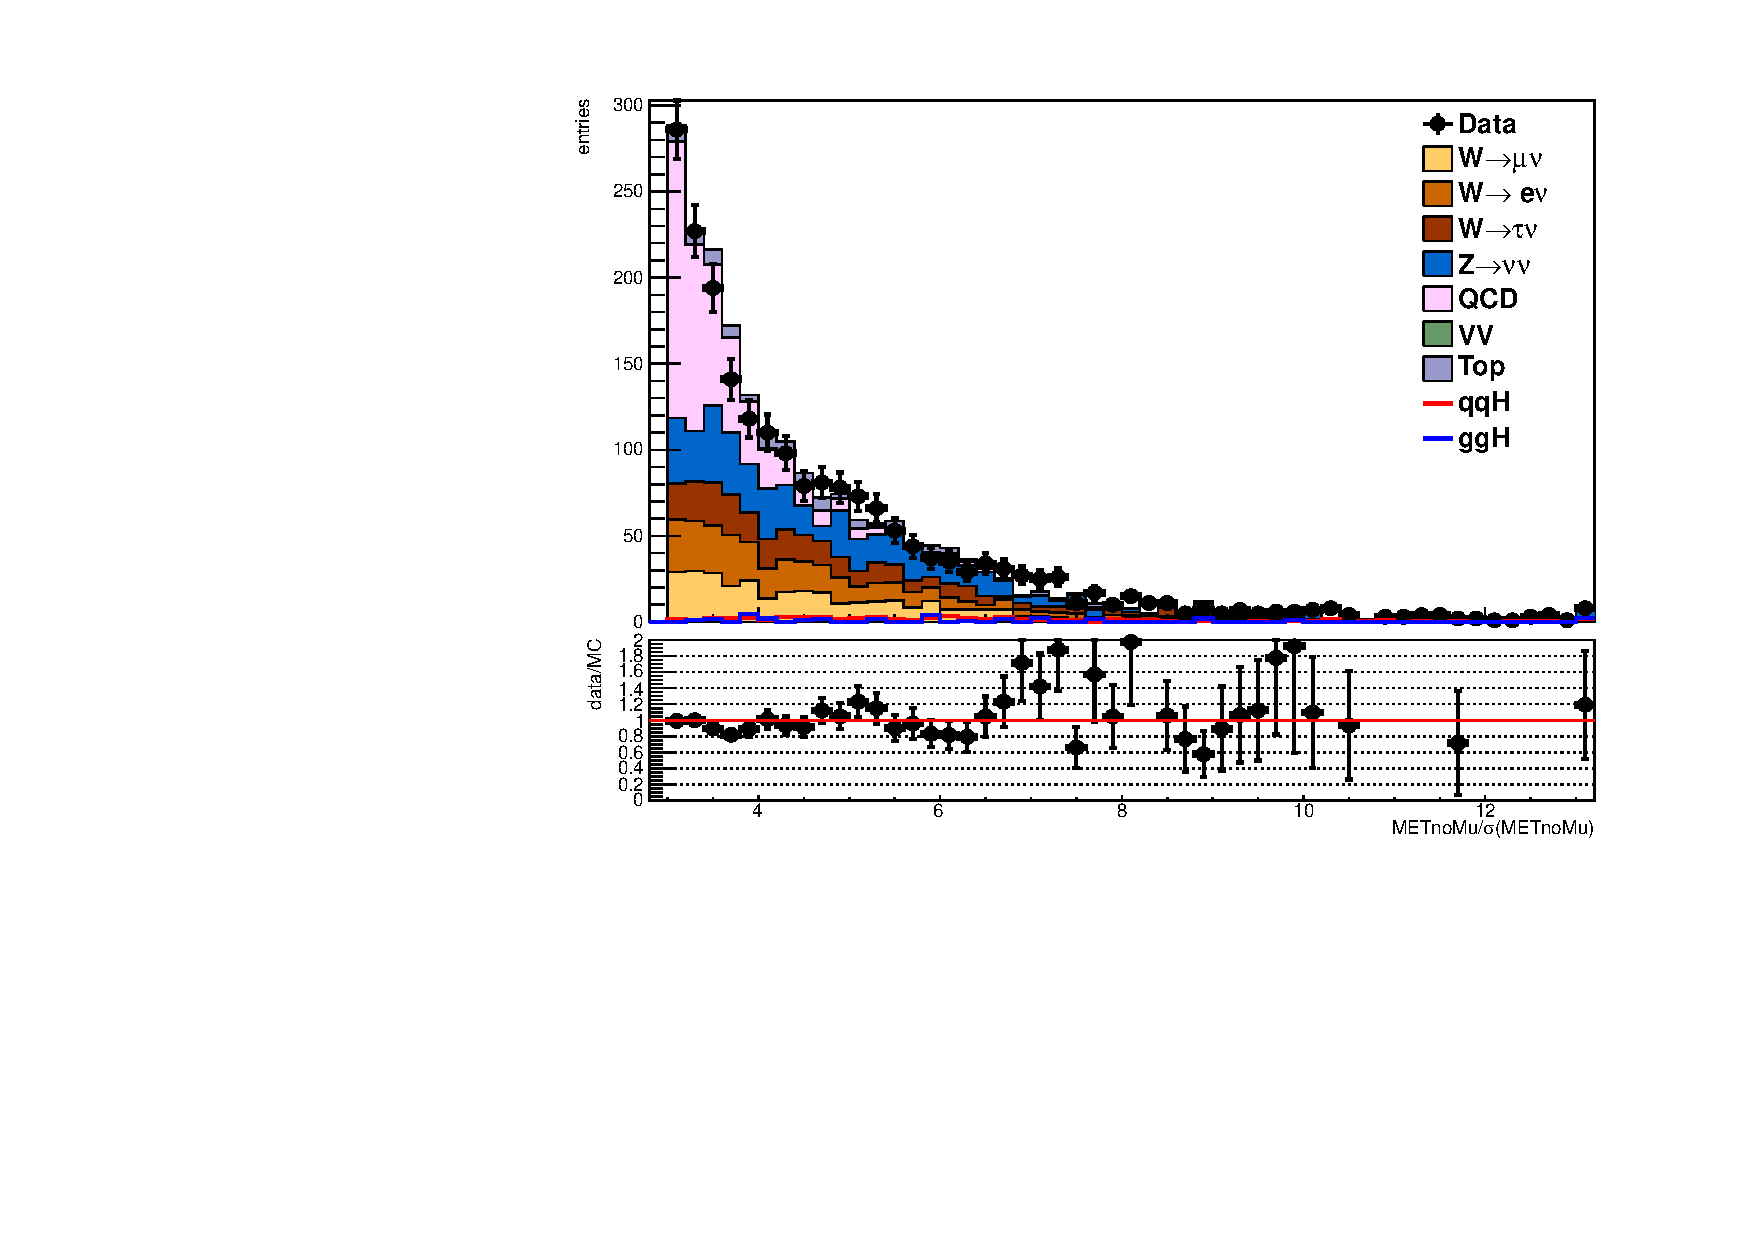
\includegraphics[width=0.5\textwidth]{./qcdinv_3j_nunu_metnomu_significance.pdf}
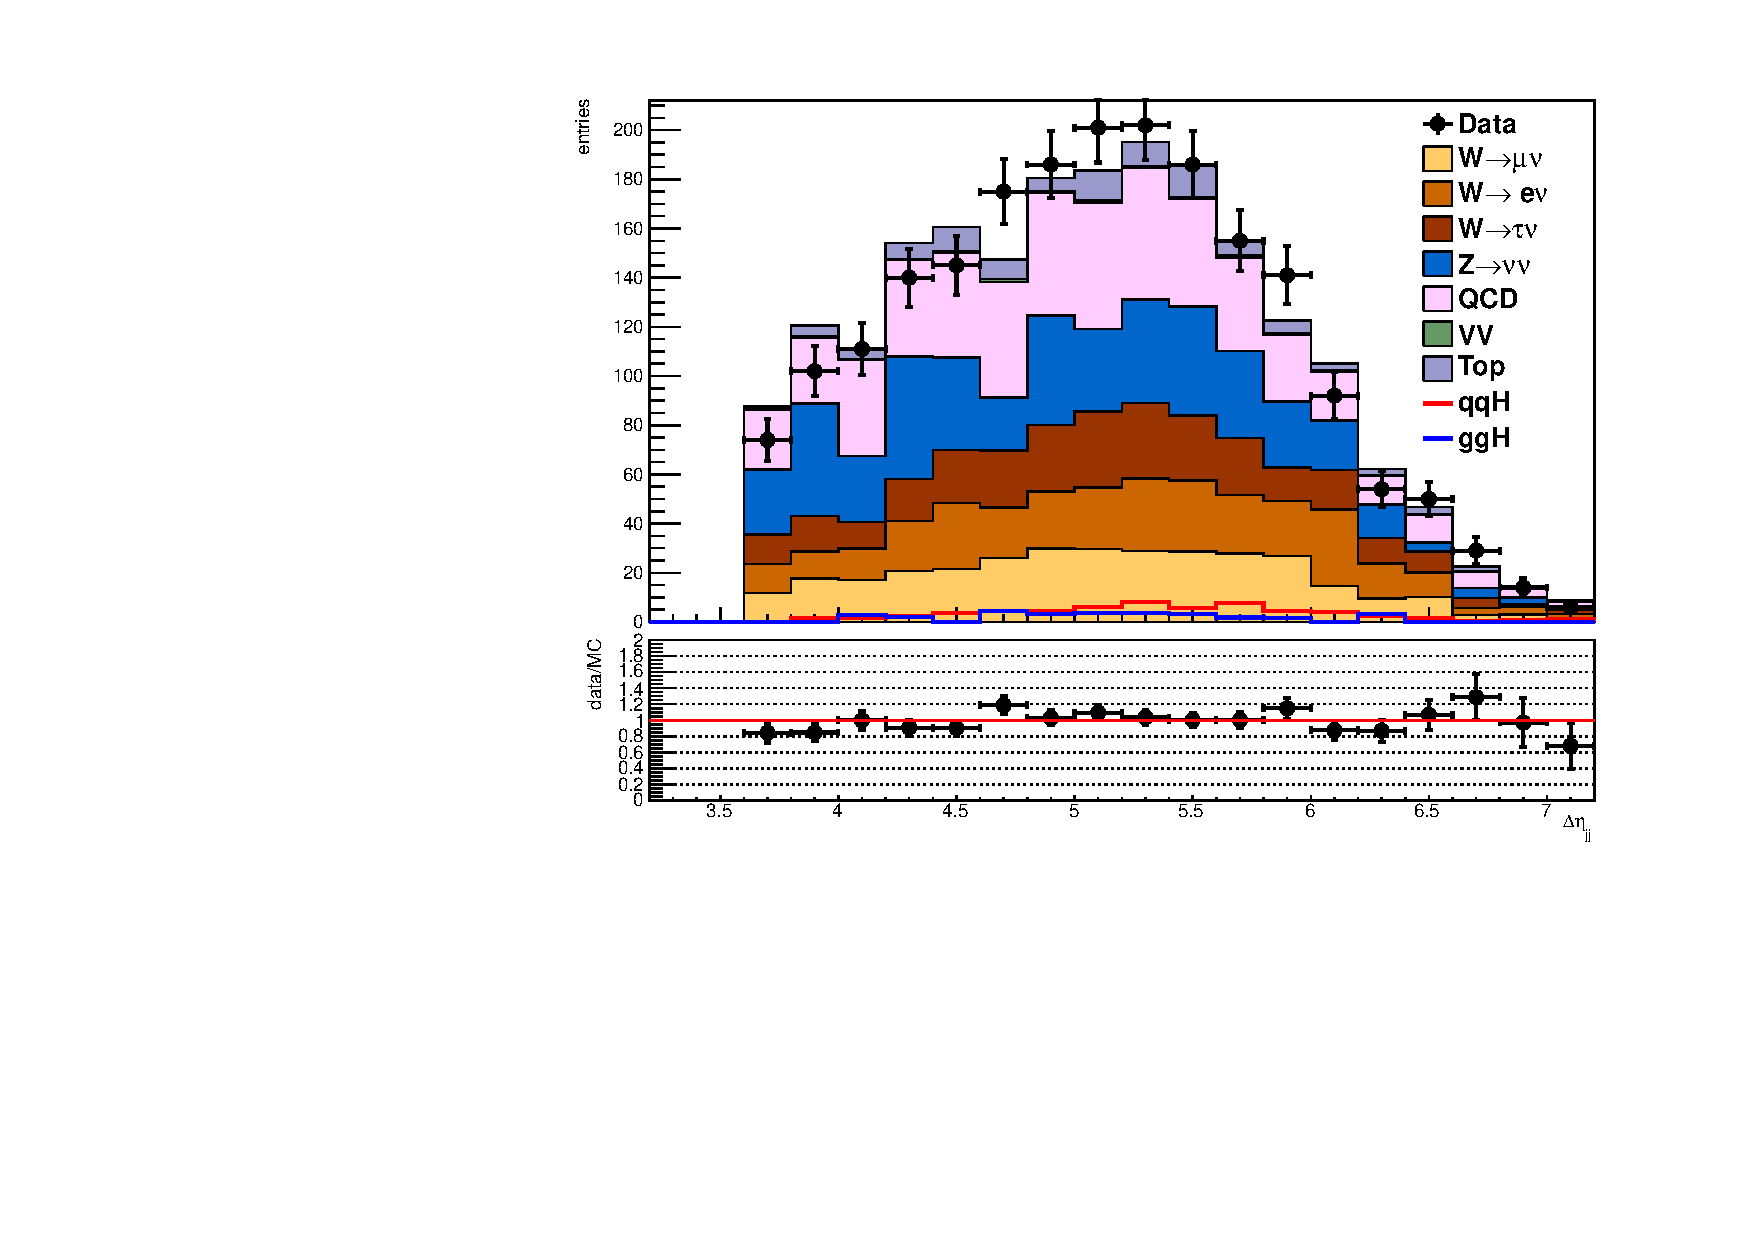
\includegraphics[width=0.5\textwidth]{./qcdinv_3j_nunu_dijet_deta.pdf}
\end{block}
\end{columns}


\end{frame}

\begin{frame}
\frametitle{Results}

\begin{columns}
  \column{0.5\textwidth}
{\tiny
  \begin{tabular}{|l|c|}
    \hline
    Background       & $N_{est} \pm (stat) \pm (syst)$ \\
    \hline
    $Z\rightarrow\nu\nu$&$157.3 \pm 37.6 \pm 38.3$\\
    $W\rightarrow\mu\nu$&$101.8 \pm 6.1 \pm 11.9$\\
    $W\rightarrow e\nu$&$57.4 \pm 7.3 \pm 7.0$\\
    $W\rightarrow\tau\nu$&$98.0 \pm 13.2 \pm 25.4$\\
    top&$4.4 \pm 1.0 \pm 1.4$\\
    VV&$3.8 \pm 0.0 \pm 0.7$\\
    QCD multijet &$17\pm 0 \pm14$\\
    \hline
    Total Background &$439.7 \pm 41.0 \pm 55.8 $\\
    \hline
    Signal(VBF) &$273.4 \pm 0.0 \pm 31.2 $\\
    Signal(ggH) &$22.6 \pm 0.0 \pm 15.6 $\\
    \hline
    Data observed & 508 \\
    \hline
  \end{tabular}
}  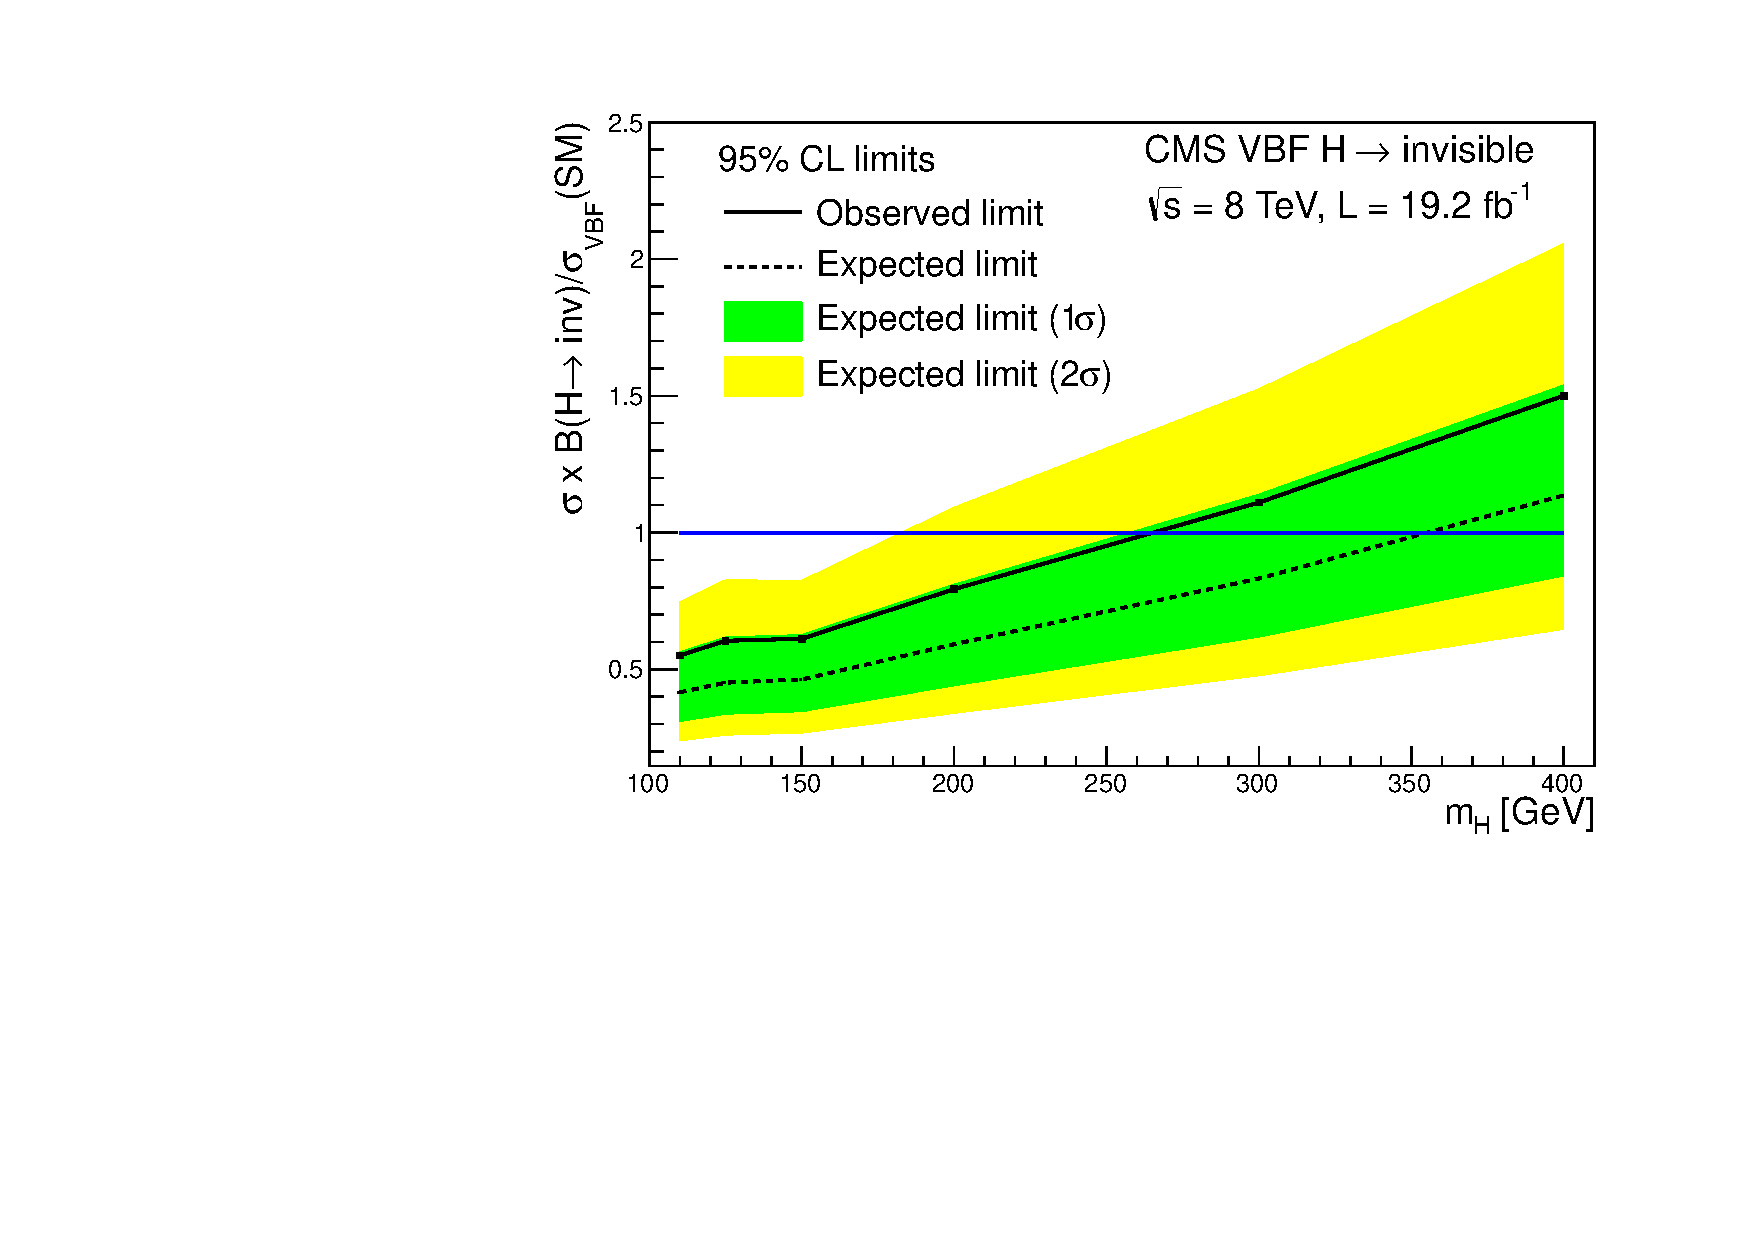
\includegraphics[width=1.0\textwidth]{./vbflimit.pdf}
  \column{0.5\textwidth}
  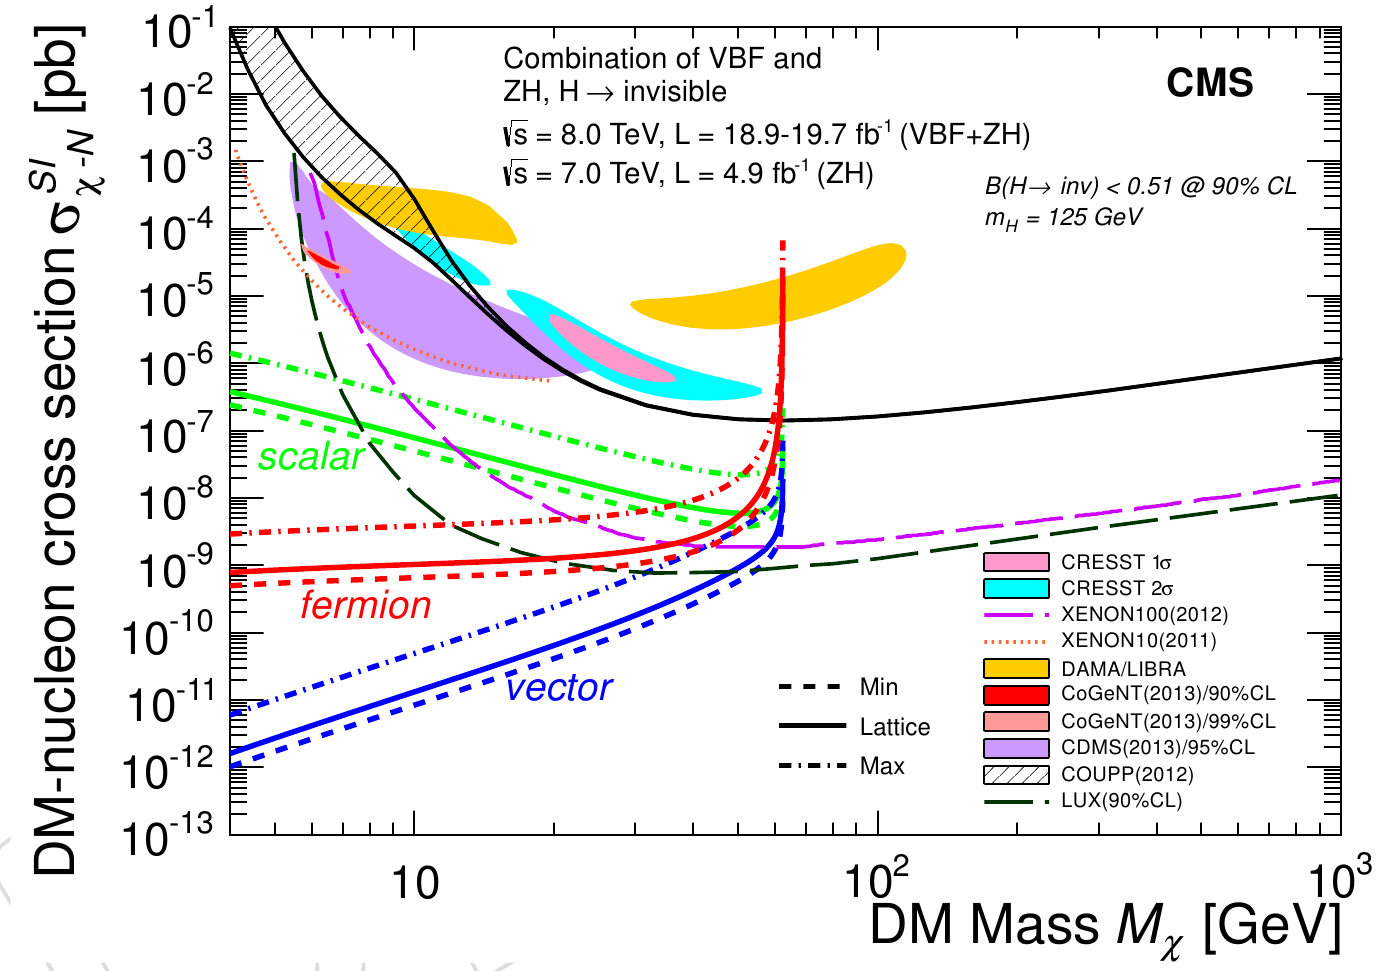
\includegraphics[width=1.0\textwidth]{./DMlimits.png}
\end{columns}

\end{frame}

\begin{frame}
\frametitle{Goals of the long exercise}

\begin{itemize}
\item \scriptsize Analyse 13 TeV MC starting from miniAOD samples.
\item \scriptsize Re-optimise selection with new trigger MET threshold. 
\item \scriptsize Extract expected yields for W(e,$\mu$,$\tau$) and Z.
\item \scriptsize Extract 95\% confidence limits on branching ratio Higgs$\rightarrow$invisible for m$_H=125$ GeV, as function of Run II luminosity.
\item \scriptsize Interpret limit in Dark Matter models.
\end{itemize}

\end{frame}

\begin{frame}
\frametitle{Proposed list of tasks}

\begin{itemize}
\item \scriptsize MiniAOD -> LightTree step.
\item \scriptsize Trigger: VBF trigger not available yet, apply threshold by hand on L1MET (known to be dominant component of the turn-on).
\item \scriptsize Selection: apply trigger-driven and QCD-killer selections.
\item \scriptsize Use Run I scale factors control->signal regions for W,Z,top.
\item \scriptsize Use TMVA cut-based optimisation on 5 variables: MET significance, min$\Delta\phi$(all jets p$_T>30$ GeV, MET), p$_T^{jets}$, M$_{jj}$using W/Z vs signal: choose point with highest purity (should translate to best 95\% CL limit).
\item \scriptsize Study dependence to pile-up on signal sample: efficiency vs number of vertices to check impact of PU jetID in 25ns scenario.
\item \scriptsize Plots of main kinematic variables, in control and signal regions.
\item \scriptsize Table of expected yields in control and signal region for 10 fb$^{-1}$.
\item \scriptsize Expected 95\% limit on BR using systematics from run I, for m$_H=125$ GeV, extrapolated to different integrated luminosity.
\item \scriptsize Conversion to DM models.
\end{itemize}

\end{frame}


\end{document}


